\documentclass[12pt,a4paper]{article}

% ==================== 宏包加载 ====================
\usepackage[UTF8]{ctex}           % 中文支持
\usepackage[margin=2.5cm]{geometry} % 页边距
\usepackage{graphicx}             % 图片支持
\usepackage{float}                % 图片位置控制 [H]
\usepackage{hyperref}             % 超链接
\usepackage{listings}             % 代码高亮
\usepackage{xcolor}               % 颜色定义
\usepackage{fancyhdr}             % 页眉页脚
\usepackage{titlesec}             % 标题格式
\usepackage{enumitem}             % 列表间距控制
\usepackage{booktabs}             % 三线表
\usepackage{array}                % 表格增强
\usepackage{caption}              % 图表标题增强
\usepackage{tcolorbox}            % 彩色文本框
\usepackage{fontawesome5}         % 图标 (若编译报错可注释掉并替换图标)
\usepackage{tabularx}             % 自适应表格
\usepackage{setspace}             % 行距
\usepackage{tikz}                 % 绘图 (用于装饰)

% ==================== 浅蓝色主题颜色定义 ====================
\definecolor{themeBlue}{RGB}{70, 130, 180}       % 钢蓝色 (主色调)
\definecolor{lightBlueBg}{RGB}{230, 240, 255}    % 极浅蓝 (背景)
\definecolor{codeBlue}{RGB}{240, 248, 255}       % 爱丽丝蓝 (代码背景)
\definecolor{darkText}{RGB}{30, 30, 30}          % 深灰黑 (正文)
\definecolor{accentBlue}{RGB}{100, 149, 237}     % 矢车菊蓝 (强调)

% ==================== 全局字体设置 (自动适配系统) ====================
% 注意：不再手动指定 SimSun，让 ctex 根据操作系统自动选择，避免 "Font not found" 错误
% 如果需要英文衬线体，可保留下面这行，否则注释掉
% \setmainfont{Times New Roman} 

% ==================== 代码样式配置 (浅蓝风格) ====================
\lstdefinestyle{mystyle}{
    language=bash,
    backgroundcolor=\color{codeBlue},   % 浅蓝背景
    basicstyle=\ttfamily\small\color{darkText},
    commentstyle=\color{gray}\itshape,
    keywordstyle=\color{themeBlue}\bfseries, % 关键字用主题蓝
    stringstyle=\color{accentBlue},
    breakatwhitespace=false,
    breaklines=true,
    captionpos=b,
    keepspaces=true,
    numbers=none,
    numbersep=8pt,
    numberstyle=\tiny\color{themeBlue}, % 行号用主题蓝
    showspaces=false,
    showstringspaces=false,
    showtabs=false,
    tabsize=2,
    frame=single,                       % 单线边框
    rulecolor=\color{themeBlue},        % 边框颜色
    framerule=1pt,
    xleftmargin=1em,
    framexleftmargin=0.5em,
    framextopmargin=4pt,
    framexbottommargin=4pt,
    aboveskip=1em,
    belowskip=1em,
    literate={~} {$\sim$}{1}            % 处理波浪号显示
}
\lstset{style=mystyle}

% ==================== 页眉页脚 ====================
\pagestyle{fancy}
\fancyhf{}
\fancyhead[L]{\small\color{themeBlue} \textbf{系统开发工具基础 · 实验报告}}
\fancyhead[R]{\small\color{gray} 洪朦朦 \quad 24170001032}
\fancyfoot[C]{\thepage}
\renewcommand{\headrulewidth}{0.4pt}
\renewcommand{\headrule}{\color{themeBlue}\hrule} % 页眉线也是蓝色

% ==================== 自定义文本框 (tcolorbox) ====================
% 思路框 (浅蓝底)
\newtcolorbox{infobox}[1][]{
    colback=lightBlueBg,
    colframe=themeBlue,
    fonttitle=\bfseries\color{white},
    coltitle=white,
    title={#1},
    rounded corners,
    boxrule=0.5pt,
    left=5pt, right=5pt, top=5pt, bottom=5pt
}

% 重点框 (稍深蓝边框)
\newtcolorbox{keybox}[1][]{
    colback=white,
    colframe=accentBlue,
    fonttitle=\bfseries\color{themeBlue},
    title={#1},
    rounded corners,
    boxrule=1pt,
    left=5pt, right=5pt, top=5pt, bottom=5pt
}

% ==================== 图片占位符命令 ====================
\newcommand{\imgplaceholder}[2][0.8\textwidth]{%
    \begin{figure}[H]
        \centering
        \fboxrule=1pt \fboxsep=10pt
        \fcolorbox{themeBlue}{lightBlueBg}{%
            \parbox{#1}{\centering\vspace{2cm}
                {\color{themeBlue}\Large\faImage}\\[0.2cm]
                {\small\color{gray} #2}\\[0.2cm]
                \vspace{2cm}
            }%
        }
        \captionsetup{labelfont={color=themeBlue,bf}, textfont={color=darkText}}
        \caption{#2}
        \label{fig:#2}
    \end{figure}
}

% ==================== 文档元数据 ====================
\newcommand{\myname}{洪朦朦}
\newcommand{\myid}{24170001032}
\newcommand{\myteacher}{周小伟}
\newcommand{\myrepo}{https://github.com/88594959h/Assignment\_for\_System\_Development\_Tools}
\newcommand{\reportdate}{\today}

% ==================== 标题格式定制 ====================
\titleformat{\section}
  {\Large\bfseries\color{themeBlue}}
  {\thesection}
  {1em}
  {}
  [\titlerule] % 标题下加蓝线

\titleformat{\subsection}
  {\large\bfseries\color{accentBlue}}
  {\thesubsection}
  {1em}
  {}

\titleformat{\subsubsection}
  {\normalsize\bfseries\color{darkText}}
  {\thesubsubsection}
  {1em}
  {}

\begin{document}

% ==================== 封面 ====================
\begin{titlepage}
    \centering
    \vspace*{2cm}
    
    % 顶部装饰线
    {\color{themeBlue}\rule{\textwidth}{2pt}}
    \vspace{1cm}
    
    {\fontsize{28}{36}\selectfont\bfseries\color{themeBlue} 系统开发工具基础}
    \vspace{0.5cm}
    
    {\fontsize{20}{28}\selectfont\bfseries\color{darkText} 第 2 周实验报告}
    
    \vspace{2cm}
    
    % 信息表格
\begin{tabularx}{\textwidth}{@{}lX@{}}
    {\large\textbf{课程名称：}} & {\large 系统开发工具基础} \\[12pt]
    {\large\textbf{授课教师：}} & {\large \myteacher} \\[12pt]
    {\large\textbf{学生姓名：}} & {\large \myname} \\[12pt]
    {\large\textbf{学\qquad 号：}} & {\large \myid} \\[12pt]
    {\large\textbf{报告日期：}} & {\large \reportdate} \\[12pt]
    {\large\textbf{GitHub：}} & {\large \href{\myrepo}{\nolinkurl{\myrepo}}} \\[12pt]
\end{tabularx}
    
    \vfill
    
    % 底部装饰
    {\color{themeBlue}\rule{\textwidth}{2pt}}
    \vspace{1cm}
    {\small\color{gray} 计算机科学与技术学院 \quad 2026年}
    
\end{titlepage}

% ==================== 实验概述 ====================
\section{实验概述}

\subsection{实验环境}
\begin{itemize}[leftmargin=2em, itemsep=5pt]
    \item \textbf{操作系统}：Windows 11 + Git Bash (MINGW64)
    \item \textbf{Shell}：Bash (Git for Windows)
    \item \textbf{版本控制}：Git 2.x
    \item \textbf{\LaTeX{} 发行版}：TeX Live 2024+
    \item \textbf{编辑器}：VS Code
\end{itemize}

\subsection{GitHub 仓库信息}
\begin{itemize}[leftmargin=2em]
    \item \textbf{仓库地址}：\href{\myrepo}{\myrepo}
\end{itemize}

\begin{figure}[H]
    \centering
    
\includegraphics[width=0.9\textwidth]{commit_log.png}
    \captionsetup{labelfont={color=themeBlue,bf}, textfont={color=darkText}}
    \caption{Git Commit 历史记录截图（git log --oneline）}
    \label{fig:commit_log}
\end{figure}

% ==================== 课上实验部分 ====================
\newpage
\section{课上实验 (第 2 周)}

% ---------- 实验一 ----------
\subsection{实验一：控制一个可清理的后台任务}

\subsubsection{题目要求}
\begin{enumerate}[leftmargin=2em]
    \item 将给定脚本保存为 \texttt{q05/worker.sh}，赋予执行权限，在前台启动并将 stdout、stderr 分别写入 \texttt{stdout.log}、\texttt{stderr.log}。
    \item 使用 Ctrl-Z 挂起任务，再用 \texttt{bg} 让其在后台继续运行；使用 \texttt{jobs} 确认状态。
    \item 使用 \texttt{jobs -p} 或等价方式动态取得 PID（不得手工抄写），发送 SIGTERM 并等待任务结束。
    \item 确认 \texttt{cleanup.log} 中出现 \texttt{CLEAN\_EXIT}，且任务已正常退出；禁止使用 \texttt{kill -9}。
\end{enumerate}

\subsubsection{核心指令与实现}
\begin{lstlisting}[caption={实验一关键 Shell 指令}]
#1.生成脚本
$ cat > worker.sh << 'EOF'
> #!/usr/bin/env bash
trap 'echo CLEAN_EXIT >> cleanup.log; exit 0' TERM INT
n=0
while true; do
    echo "$n"
    n=$((n+1))
    sleep 1
done
EOF

#2.赋予权限
$ chmod +x worker.sh

#3.前台启动并重定向日志
$ ./worker.sh >stdout.log 2>stderr.log

#4.在终端按 Ctrl-Z 挂起后，后台继续，确认状态
$ bg %1  
$ jobs 

#5.动态获取 PID 并发送 SIGTERM
$ PID=$(jobs -p)
$ kill -TERM "$PID"
$ wait "$PID" 

#6.验证清理结果
$ grep "CLEAN_EXIT" cleanup.log
$ jobs 
$ ps -p "$PID"  
\end{lstlisting}

\subsubsection{实验分析}
\begin{infobox}[实现思路]
准备阶段创建脚本并赋权，以前台模式启动且分离重定向 stdout 与 stderr；通过 Ctrl-Z 挂起进程后使用 \texttt{bg} 转入后台，并用 \texttt{jobs} 验证状态；利用 \texttt{jobs -p} 动态获取 PID 发送 SIGTERM 触发 \texttt{trap} 清理机制，最后用 \texttt{wait} 等待退出并验证 \texttt{cleanup.log} 中的标记。
\end{infobox}
\paragraph{实验重点}
\begin{itemize}[leftmargin=2em]
    \item \textbf{I/O 重定向语法}：掌握 \texttt{>stdout.log 2>stderr.log} 分别重定向 stdout (fd=1) 和 stderr (fd=2) 的写法。
    \item \textbf{作业控制三件套}：理解 Ctrl-Z（挂起）、\texttt{bg}（后台继续）、\texttt{jobs}（查看状态）的协作流程。
    \item \textbf{动态 PID 获取}：必须使用 \texttt{jobs -p} 或 \texttt{\$!} 等 shell 内置机制获取 PID，严禁手动复制粘贴数字。
    \item \textbf{Trap 信号处理}：理解 \texttt{trap '...' TERM INT} 的作用——捕获 SIGTERM/SIGINT 后执行清理逻辑再退出，这是实现“可清理”的核心。
    \item \textbf{优雅退出 vs 强制杀死}：区分 SIGTERM（允许进程自行清理）与 SIGKILL/\texttt{kill -9}（立即终止、无法被 trap 捕获）的本质区别。
\end{itemize}

\subsubsection{运行结果}
\begin{figure}[H]
    \centering
    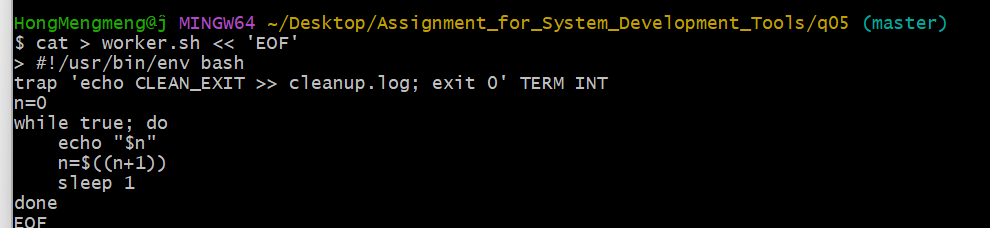
\includegraphics[width=0.9\textwidth]{实验一生成脚本.png}
    \captionsetup{labelfont={color=themeBlue,bf}, textfont={color=darkText}}
    \caption{实验一：生成脚本}
\end{figure}

\begin{figure}[H]
    \centering
    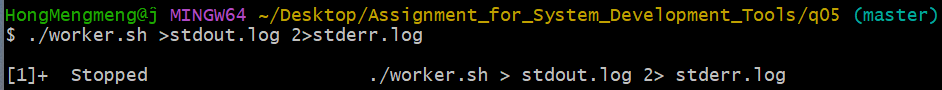
\includegraphics[width=0.9\textwidth]{实验一重定向日志.png}
    \captionsetup{labelfont={color=themeBlue,bf}, textfont={color=darkText}}
    \caption{实验一：重定向日志}
\end{figure}

\begin{figure}[H]
    \centering
    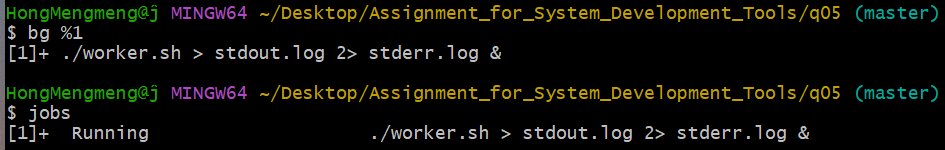
\includegraphics[width=0.9\textwidth]{实验一挂起并确认状态.png}
    \captionsetup{labelfont={color=themeBlue,bf}, textfont={color=darkText}}
    \caption{实验一：挂起并确认状态}
\end{figure}

\begin{figure}[H]
    \centering
    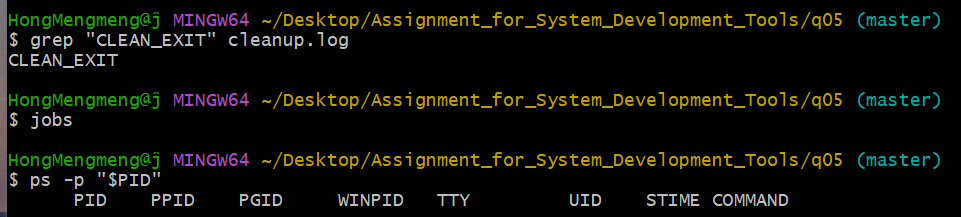
\includegraphics[width=0.9\textwidth]{验证清理结果.png}
    \captionsetup{labelfont={color=themeBlue,bf}, textfont={color=darkText}}
    \caption{实验一：验证清理结果}
\end{figure}

%----------实验二-----------
\subsection{实验二：语义重构与本地开发反馈}

\subsubsection{题目要求}
\begin{enumerate}[leftmargin=2em]
    \item 在已配置好 Python、pytest 和 ruff 的课程环境中打开 \texttt{q06} 目录，并启用 Python 语言服务器；按照给定内容分别创建 \texttt{math\_utils.py}、\texttt{app.py} 和 \texttt{test\_math\_utils.py} 三个文件。
    \item 使用编辑器语言服务器功能，分别演示对符号 \texttt{total\_price} 的“跳转到定义”与“查找引用”操作。
    \item 使用“重命名符号”功能将 \texttt{total\_price} 重构为 \texttt{calculate\_total}，确保函数定义及所有跨文件引用同步更新，且无遗漏或错误。
    \item 在 \texttt{app.py} 中临时添加未使用的导入语句 \texttt{import os}，使用 \texttt{ruff} 检测该问题并自动/手动删除；最终运行 \texttt{ruff check} 与 \texttt{pytest}，确保两者均无报错并通过验证。
\end{enumerate}

\subsubsection{核心指令与实现}
\begin{lstlisting}[caption={实验二关键 Shell 指令}]
#1.创建三个Python文件
$ cat << 'EOF' > math_utils.py
def total_price(price: float, count: int) -> float:
    return price * count
EOF

$ cat << 'EOF' > app.py
from math_utils import total_price
print(total_price(12.5, 4))
EOF

$ cat << 'EOF' > test_math_utils.py
from math_utils import total_price
def test_total_price():
    assert total_price(12.5, 4) == 50.0
EOF

#2.打开代码编辑器
code .

#3. 在 app.py 顶部临时加入未使用的 import os
$ sed -i '1i import os' app.py

#4.使用 ruff 发现代码问题
$ python -m ruff check app.py

#5.使用 ruff 自动修复并删除未使用的 import
$ python -m ruff check --fix app.py

#6.验证 app.py 中的 import os 已被自动删除
$ cat app.py

#7.对整个目录运行 ruff 检查，确保无任何警告或错误
$ python -m ruff check .

#8.运行 pytest，确保测试全部通过
$ python -m pytest
\end{lstlisting}

\subsubsection{实验分析}
\begin{infobox}[实现思路]
在已配置好 Python、pytest 与 ruff 的课程环境中打开 q06 目录，创建 \texttt{math\_utils.py}、\texttt{app.py} 和 \texttt{test\_math\_utils.py} 三个文件并写入给定代码；启用编辑器的 Python 语言服务器（如 Pylance），分别演示"跳转到定义"（Go to Definition）定位到 \texttt{total\_price} 的函数体，以及"查找引用"（Find References）列出该符号在三个文件中的所有引用位置；随后使用"重命名符号"（Rename Symbol）将 \texttt{total\_price} 统一改为 \texttt{calculate\_total}，验证定义与所有引用同步更新；最后在 \texttt{app.py} 中临时添加未使用的 \texttt{import os}，运行 ruff 检测并删除该冗余导入，再次运行 ruff 与 pytest 确保全部通过。
\end{infobox}
\paragraph{实验重点}
\begin{itemize}[leftmargin=2em]
    \item \textbf{语言服务器（LSP）}：理解 Language Server Protocol 的作用——为编辑器提供语义级别的代码分析能力（跳转定义、查找引用、重命名等），远超纯文本搜索。
    \item \textbf{跳转到定义与查找引用}：掌握 Go to Definition（快速定位符号声明处）和 Find References（列出符号在所有文件中的使用位置）的操作，体会语言服务器对跨文件符号关系的精确追踪。
    \item \textbf{语义重命名 vs 文本替换}：区分"Rename Symbol"与全局查找替换的本质差异——前者基于语法树和符号作用域，仅修改同一符号的引用，不会误伤同名但不同作用域的标识符。
    \item \textbf{静态检查工具 ruff}：理解 ruff 作为 linter 的作用——在代码运行前即可发现未使用的导入（unused import）、语法问题等，帮助保持代码整洁与规范。
    \item \textbf{测试驱动的开发反馈}：体会 pytest 在重构后的回归验证价值——重命名符号后立即运行测试，确保功能行为未被破坏，形成"重构—检查—测试"的良性开发循环。
\end{itemize}

\subsubsection{运行结果}
\begin{figure}[H]
    \centering
    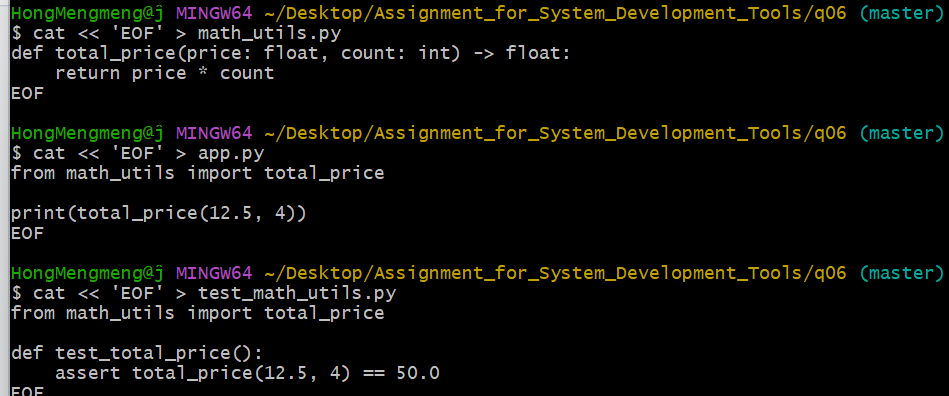
\includegraphics[width=0.9\textwidth]{实验二创建三个Python文件.png}
    \captionsetup{labelfont={color=themeBlue,bf}, textfont={color=darkText}}
    \caption{实验二:创建三个Python文件}
\end{figure}

\begin{figure}[H]
    \centering
    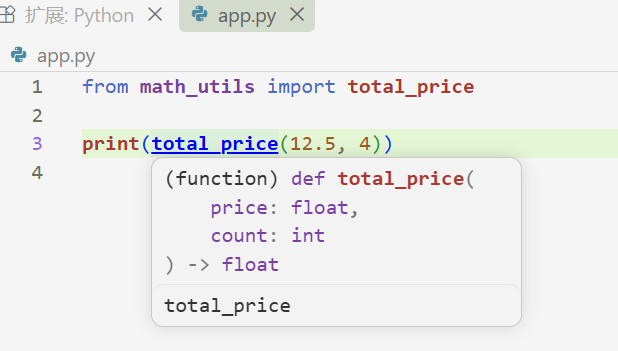
\includegraphics[width=0.9\textwidth]{实验二按住Ctrl并点击totalprice.png}
    \captionsetup{labelfont={color=themeBlue,bf}, textfont={color=darkText}}
    \caption{实验二:按住Ctrl并点击total\_price}
\end{figure}

\begin{figure}[H]
    \centering
    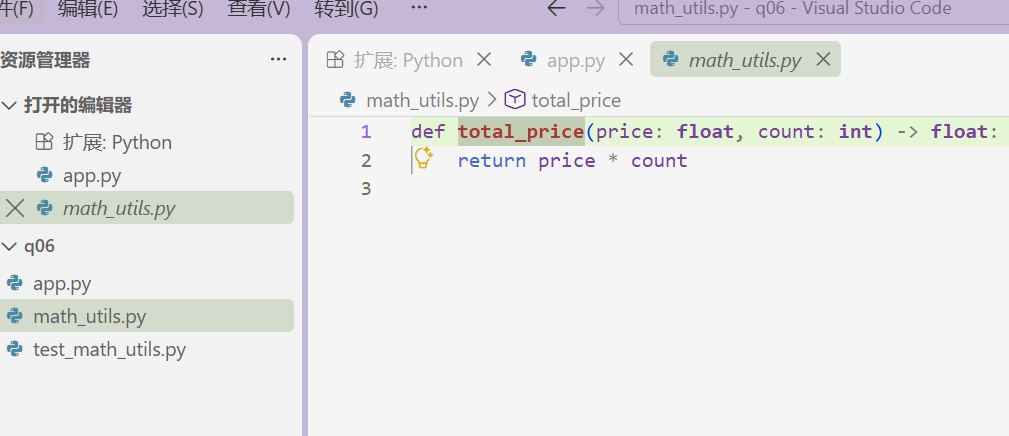
\includegraphics[width=0.9\textwidth]{实验二跳转到定义.png}
    \captionsetup{labelfont={color=themeBlue,bf}, textfont={color=darkText}}
    \caption{实验二:跳转到定义}
\end{figure}

\begin{figure}[H]
    \centering
    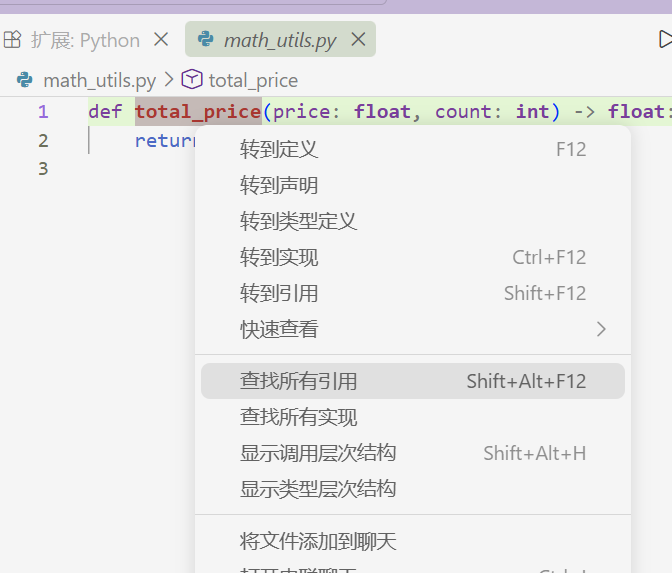
\includegraphics[width=0.9\textwidth]{实验二查找引用.png}
    \captionsetup{labelfont={color=themeBlue,bf}, textfont={color=darkText}}
    \caption{实验二:查找引用}
\end{figure}

\begin{figure}[H]
    \centering
    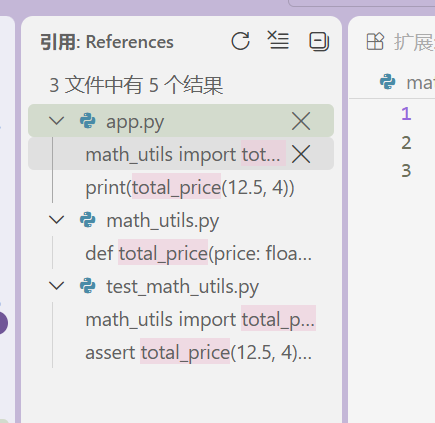
\includegraphics[width=0.9\textwidth]{实验二列出调用.png}
    \captionsetup{labelfont={color=themeBlue,bf}, textfont={color=darkText}}
    \caption{实验二:列出调用}
\end{figure}

\begin{figure}[H]
    \centering
    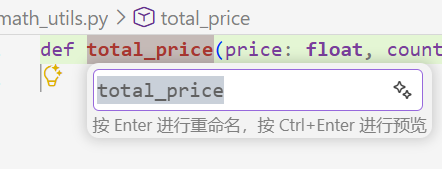
\includegraphics[width=0.9\textwidth]{实验二右键F2重命名.png}
    \captionsetup{labelfont={color=themeBlue,bf}, textfont={color=darkText}}
    \caption{实验二:右键F2重命名}
\end{figure}

\begin{figure}[H]
    \centering
    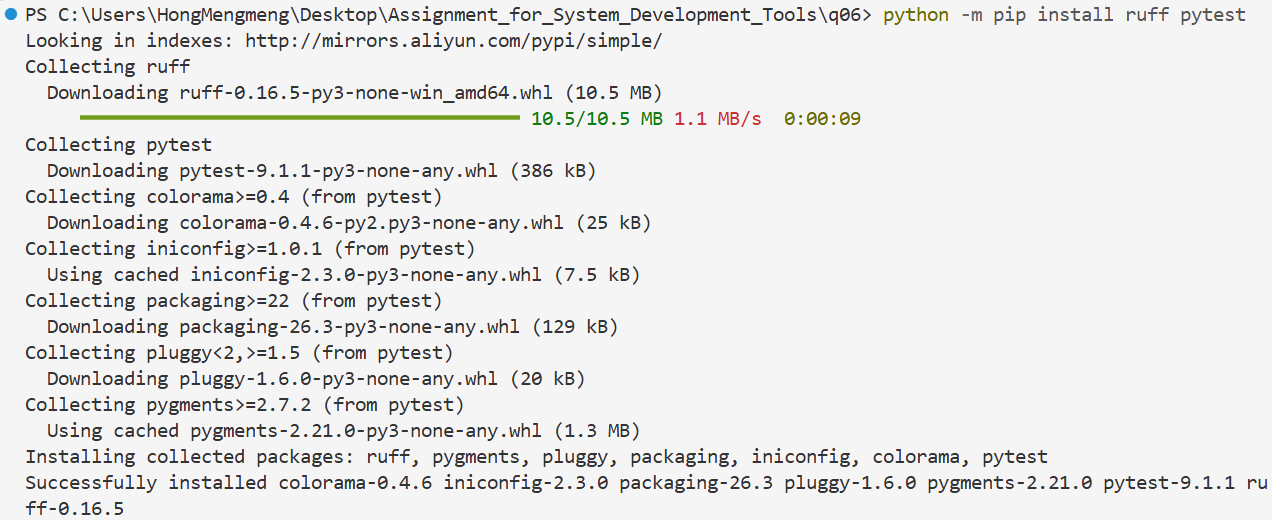
\includegraphics[width=0.9\textwidth]{实验二安装ruff和pytest插件.png}
    \captionsetup{labelfont={color=themeBlue,bf}, textfont={color=darkText}}
    \caption{实验二:安装ruff和pytest插件}
\end{figure}

\begin{figure}[H]
    \centering
    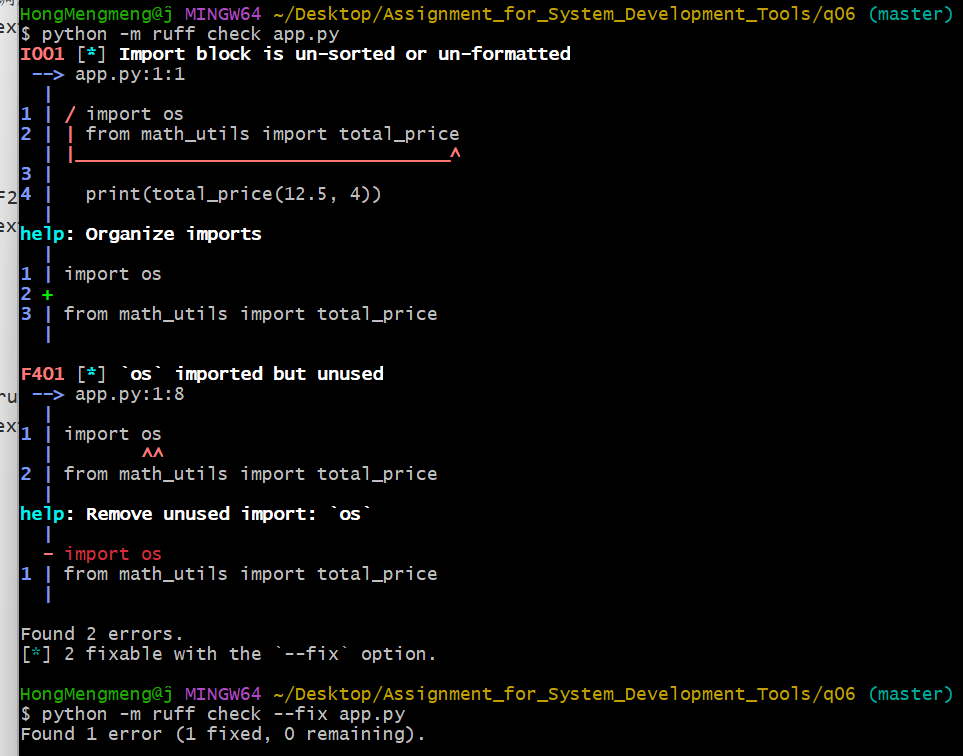
\includegraphics[width=0.9\textwidth]{实验二ruff检查并修复.png}
    \captionsetup{labelfont={color=themeBlue,bf}, textfont={color=darkText}}
    \caption{实验二:ruff检查并修复}
\end{figure}

\begin{figure}[H]
    \centering
    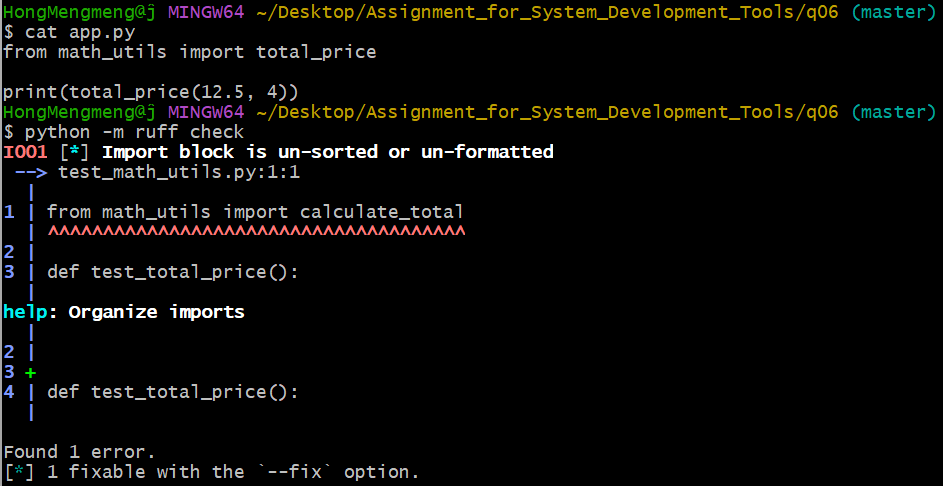
\includegraphics[width=0.9\textwidth]{实验二验证并对整个目录进行ruff检查.png}
    \captionsetup{labelfont={color=themeBlue,bf}, textfont={color=darkText}}
    \caption{实验二:验证并对整个目录进行ruff检查}
\end{figure}

\begin{figure}[H]
    \centering
    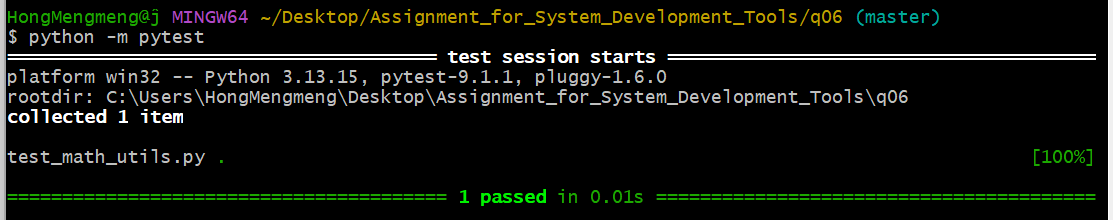
\includegraphics[width=0.9\textwidth]{实验二运行pytest确保测试通过.png}
    \captionsetup{labelfont={color=themeBlue,bf}, textfont={color=darkText}}
    \caption{实验二:运行pytest确保测试通过}
\end{figure}

% ---------- 实验三 ----------
\subsection{实验三：用调试器定位归并排序缺陷}

\subsubsection{题目要求}
\begin{enumerate}[leftmargin=2em]
\item 将给定的存在缺陷的归并排序代码保存为指定文件，先运行给定输入数据，确认程序输出结果错误或出现异常。
\item 使用调试器在合并函数中设置断点，观察左右子列表索引及对应元素值的变化过程，定位导致排序错误的具体缺陷位置。
\item 对定位到的缺陷进行最小化修复，不得直接使用内置排序函数替换原有的归并排序实现逻辑。
\item 使用测试框架增加两个测试用例，分别覆盖给定输入和含重复元素的列表，确保所有测试均能顺利通过。
\end{enumerate}

\subsubsection{核心指令与实现}
\begin{lstlisting}[caption={实验三关键 Shell 指令}]
#1.创建Python文件
$ cat << 'EOF' > merge_sort.py
> def merge(left, right):
    result = []
    i = j = 0
    while i < len(left) and j < len(right):
        if left[i] <= right[j]:
            result.append(left[i]); i += 1
        else:
            result.append(right[i]); j += 1  # 此处存在缺陷
    return result + left[i:] + right[j:]

def merge_sort(a):
    if len(a) <= 1: return a
    m = len(a) // 2
    return merge(merge_sort(a[:m]), merge_sort(a[m:]))

print(merge_sort([3, 1, 4, 1, 5, 9, 2, 6]))
> EOF

#2.运行缺陷代码，确认报错
$ python q07/merge_sort.py

#3.用 pdb 调试
$ python -m pdb q07/merge_sort.py

#4.逐条输入
$ b 8
c
p i, j, left, right
p right[i]
n
p i, j
q

#5.修复:right[i] → right[j]
$ sed -i 's/result\.append(right\[i\])/result.append(right[j])/' q07/merge_sort.py

#6.验证修复结果
$ python q07/merge_sort.py

#7创建测试文件
$ python -c "open('q07/test_merge_sort.py','w').write('from merge_sort import merge_sort\n\ndef test_given_input():\n    assert merge_sort([3, 1, 4, 1, 5, 9, 2, 6]) == [1, 1, 2, 3, 4, 5, 6, 9]\n\ndef test_duplicates():\n    assert merge_sort([5, 3, 3, 1, 5, 2, 1, 4, 4, 2]) == [1, 1, 2, 2, 3, 3, 4, 4, 5, 5]\n')"

#8.运行测试
$ cd q07
pytest test_merge_sort.py -v
\end{lstlisting}

\subsubsection{实验分析}
\begin{infobox}[实现思路]
先原样运行缺陷代码，观察输出与预期的偏差以确认 bug 存在；随后在 \texttt{merge} 函数的 \texttt{while} 循环体内设置断点，逐次检查 \texttt{i}、\texttt{j}、\texttt{left[i]}、\texttt{right[j]} 的值，发现 \texttt{else} 分支误用 \texttt{right[i]} 而非 \texttt{right[j]} 导致索引越界或取值错误；将下标 \texttt{i} 改为 \texttt{j} 完成最小修复；最后用 \texttt{pytest} 编写覆盖"给定输入"与"含重复元素"两类场景的测试，验证排序结果的正确性与稳定性。
\end{infobox}
\paragraph{实验重点}
\begin{itemize}[leftmargin=2em]
    \item \textbf{断点调试流程}：掌握在 \texttt{pdb} 中使用 \texttt{b <行号>} 设断点、\texttt{n}（单步）、\texttt{c}（继续）、\texttt{p <表达式>}（打印变量）的基本操作，能在循环中观察索引与数组元素的对应关系。
    \item \textbf{索引变量一致性}：归并排序的 \texttt{merge} 阶段使用双指针 \texttt{i}、\texttt{j} 分别遍历左右子数组，取值时必须"各用各的下标"——\texttt{left[i]} 与 \texttt{right[j]}，混淆下标是本题缺陷的根源。
    \item \textbf{最小修复原则}：仅修改出错的一个字符（\texttt{right[i]} $\to$ \texttt{right[j]}），不重构、不替换算法，体现"定位→确认→精准修改"的调试纪律。
    \item \textbf{pytest 测试设计}：使用 \texttt{assert merge\_sort(...) == expected} 进行断言；测试用例应覆盖一般乱序与大量重复元素两种情况，验证排序的\textbf{正确性}与\textbf{稳定性}。
    \item \textbf{归并排序分治结构}：理解 \texttt{merge\_sort} 递归拆半、\texttt{merge} 双指针合并的协作关系，确保修复不破坏 $O(n\log n)$ 的时间复杂度。
\end{itemize}

\subsubsection{运行结果}
\begin{figure}[H]
    \centering
    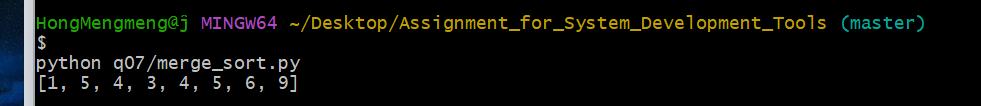
\includegraphics[width=0.9\textwidth]{实验三缺陷代码错误排序结果.png}
    \captionsetup{labelfont={color=themeBlue,bf}, textfont={color=darkText}}
    \caption{实验三:缺陷代码错误排序结果}
\end{figure}

\begin{figure}[H]
    \centering
    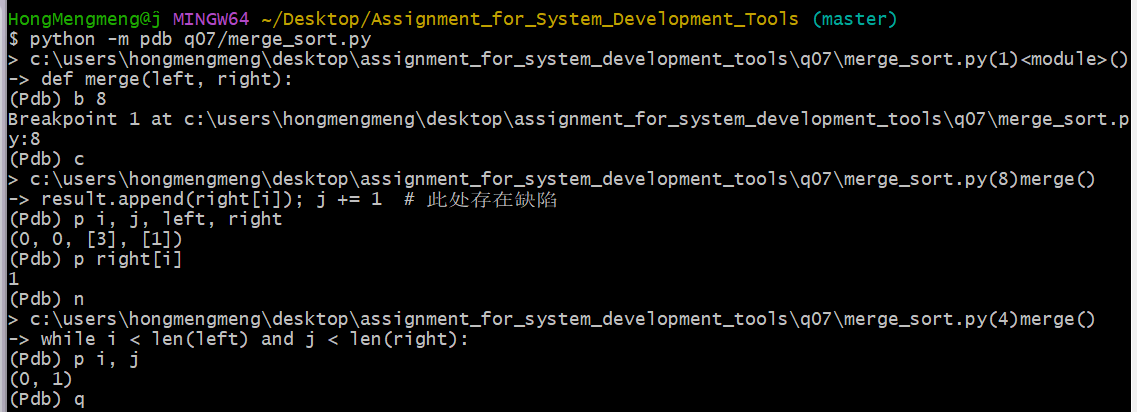
\includegraphics[width=0.9\textwidth]{实验三pdb调试过程.png}
    \captionsetup{labelfont={color=themeBlue,bf}, textfont={color=darkText}}
    \caption{实验三:pdb调试过程}
\end{figure}

\begin{figure}[H]
    \centering
    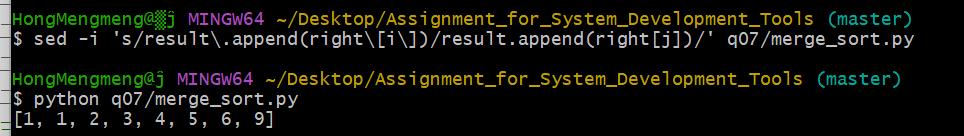
\includegraphics[width=0.9\textwidth]{实验三修复并运行.png}
    \captionsetup{labelfont={color=themeBlue,bf}, textfont={color=darkText}}
    \caption{实验三:修复并运行}
\end{figure}

\begin{figure}[H]
    \centering
    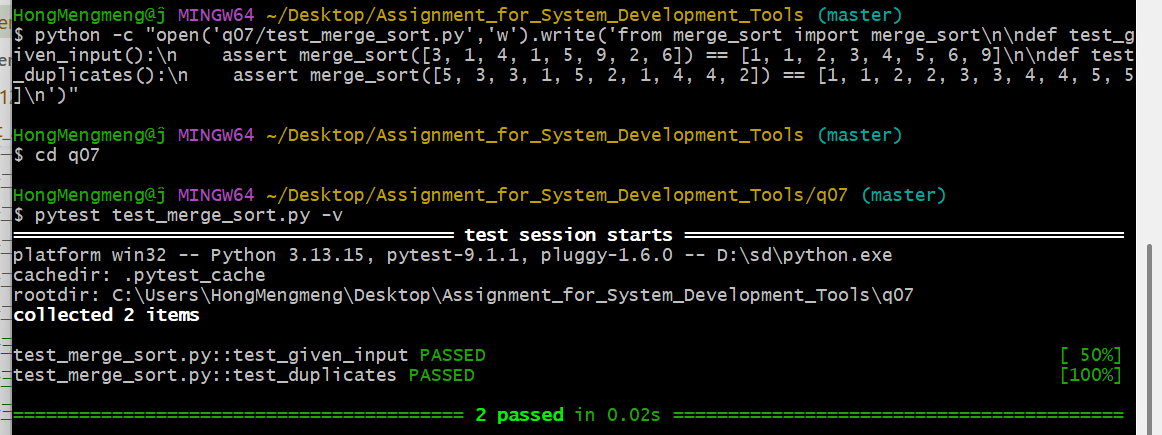
\includegraphics[width=0.9\textwidth]{实验三运行测试.png}
    \captionsetup{labelfont={color=themeBlue,bf}, textfont={color=darkText}}
    \caption{实验三:运行测试}
\end{figure}

% ---------- 实验四 ----------
\subsection{实验四：先测量，再优化慢速词频程序}

\subsubsection{题目要求}
\begin{enumerate}[leftmargin=2em]
    \item 在 \texttt{q08} 目录中创建 \texttt{generate\_words.py} 和 \texttt{wordfreq.py}，运行生成脚本产生 \texttt{words.txt}；使用 \texttt{time} 命令对原始 \texttt{wordfreq.py} 运行 2 次并记录耗时。
    \item 使用 \texttt{python -m cProfile -s cumulative wordfreq.py} 运行一次，根据累计时间排序找出主要耗时函数与行号。
    \item 在不改变最终 \texttt{count} 输出值的前提下优化程序（不得将结果硬编码为 1000），优化后使用相同输入再运行 2 次。
    \item 计算优化前后的中位数耗时及加速比（$\texttt{加速比} = \frac{\texttt{优化前中位数}}{\texttt{优化后中位数}}$），确认加速效果显著。
\end{enumerate}

\subsubsection{核心指令与实现}
\begin{lstlisting}[caption={实验四关键 Shell 指令}]
#1.创建两个Python文件
$ cat > generate_words.py << 'EOF'
import random
random.seed(20260831)
vocab = [f"w{i}" for i in range(1000)]
with open("words.txt", "w", encoding="utf-8") as f:
    f.write(" ".join(random.choice(vocab) for _ in range(30000)))
EOF

$ cat > wordfreq.py << 'EOF'
words = open("words.txt", encoding="utf-8").read().split()
unique = []
for word in words:
    if word not in unique:
        unique.append(word)
print("count=", len(unique))
EOF

#2.生成词表
$ python generate_words.py

#3.用 time 运行原程序 2 次
$ time python wordfreq.py
$ time python wordfreq.py

#4.用 cProfile 分析瓶颈
$ python -m cProfile -s cumulative wordfreq.py 

#5.优化：用 set 替代 list 做去重
$ cat > wordfreq_opt.py << 'EOF'
words = open("words.txt", encoding="utf-8").read().split()
unique = set(words)
print("count=", len(unique))
EOF

#6.用 time 运行优化后程序 2 次
$ time python wordfreq_opt.py
$ time python wordfreq_opt.py

#7创建测试文件
$ python -c "open('q07/test_merge_sort.py','w').write('from merge_sort import merge_sort\n\ndef test_given_input():\n    assert merge_sort([3, 1, 4, 1, 5, 9, 2, 6]) == [1, 1, 2, 3, 4, 5, 6, 9]\n\ndef test_duplicates():\n    assert merge_sort([5, 3, 3, 1, 5, 2, 1, 4, 4, 2]) == [1, 1, 2, 2, 3, 3, 4, 4, 5, 5]\n')"

\end{lstlisting}

\subsubsection{实验分析}
\begin{infobox}[实现思路]
首先运行 \texttt{generate\_words.py} 生成包含 30000 个随机词（词表大小 1000）的 \texttt{words.txt}；随后对原始 \texttt{wordfreq.py} 使用 \texttt{time} 计时运行 2 次，记录基线耗时；接着用 \texttt{cProfile -s cumulative} 进行性能剖析，发现瓶颈在于 \texttt{if word not in unique} 这一行——由于 \texttt{unique} 是列表，每次 \texttt{in} 查找的时间复杂度为 $O(n)$，整体循环退化为 $O(n^2)$；优化方案是将 \texttt{unique} 从 \texttt{list} 改为 \texttt{set}，利用哈希表的 $O(1)$ 平均查找将整体复杂度降至 $O(n)$；最后对优化版本同样计时 2 次，取中位数计算加速比，验证优化效果。
\end{infobox}
\paragraph{实验重点}
\begin{itemize}[leftmargin=2em]
    \item \textbf{先测量再优化（Measure First）}：遵循"不猜测瓶颈"的原则，先用 \texttt{time} 获取基线数据，再用 \texttt{cProfile} 精确定位热点函数，避免盲目优化非关键路径。
    \item \textbf{cProfile 性能剖析}：掌握 \texttt{python -m cProfile -s cumulative} 的用法——按累计时间排序输出各函数的调用次数、总耗时与单次耗时，快速锁定性能瓶颈所在行。
    \item \textbf{数据结构选择对复杂度的影响}：理解 \texttt{list} 的 \texttt{in} 操作为 $O(n)$ 线性扫描，而 \texttt{set} 基于哈希表实现 $O(1)$ 平均查找；将去重容器从列表换为集合，即可将整体算法从 $O(n^2)$ 降至 $O(n)$，这是本题加速的核心。
    \item \textbf{可重复实验设计}：使用固定随机种子（\texttt{random.seed(20260831)}）确保每次生成的 \texttt{words.txt} 完全一致，使优化前后的对比具有可重复性与公平性。
    \item \textbf{中位数与加速比}：多次运行取中位数而非均值，可减少系统抖动带来的偶然误差；加速比 $= T_{\texttt{before}} / T_{\texttt{after}}$ 是衡量优化效果的标准化指标。
\end{itemize}

\subsubsection{运行结果}
\begin{figure}[H]
    \centering
    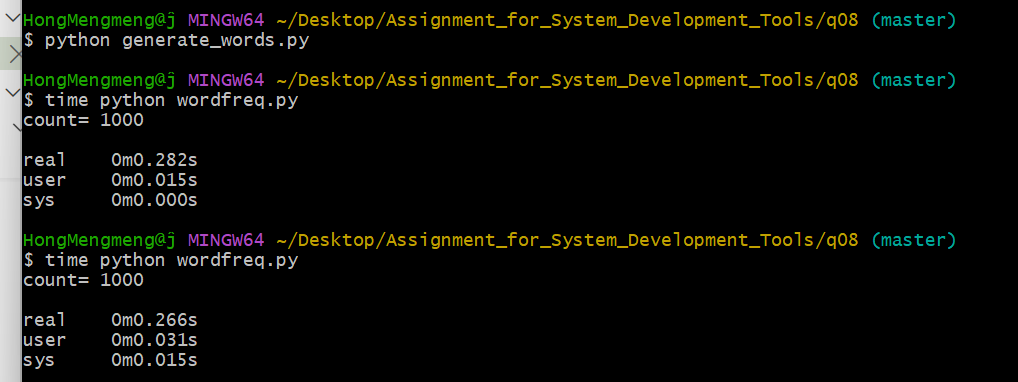
\includegraphics[width=0.9\textwidth]{实验四生成词表与原程序计时.png}
    \captionsetup{labelfont={color=themeBlue,bf}, textfont={color=darkText}}
    \caption{实验四:生成词表与原程序计时}
\end{figure}

\begin{figure}[H]
    \centering
    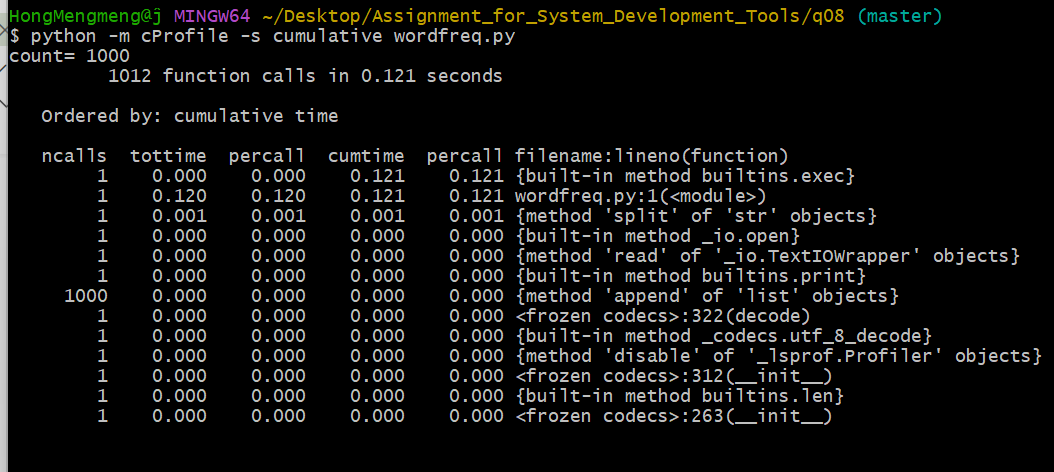
\includegraphics[width=0.9\textwidth]{实验四cProfile性能分析.png}
    \captionsetup{labelfont={color=themeBlue,bf}, textfont={color=darkText}}
    \caption{实验四:cProfile 性能分析}
\end{figure}

\begin{figure}[H]
    \centering
    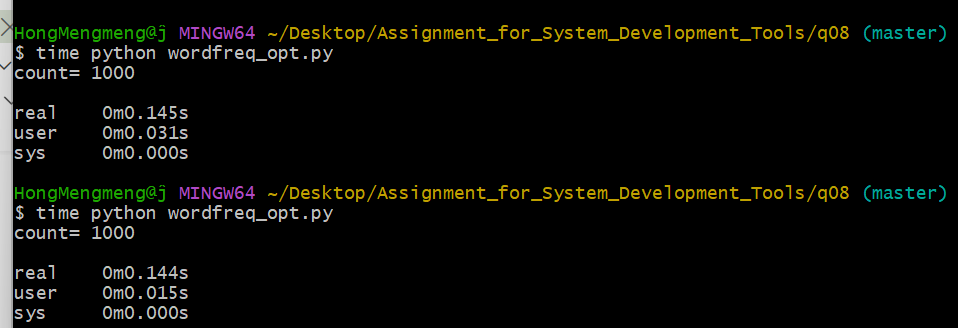
\includegraphics[width=0.9\textwidth]{实验四优化后程序计时.png}
    \captionsetup{labelfont={color=themeBlue,bf}, textfont={color=darkText}}
    \caption{实验四:优化后程序计时}
\end{figure}

\begin{figure}[H]
    \centering
    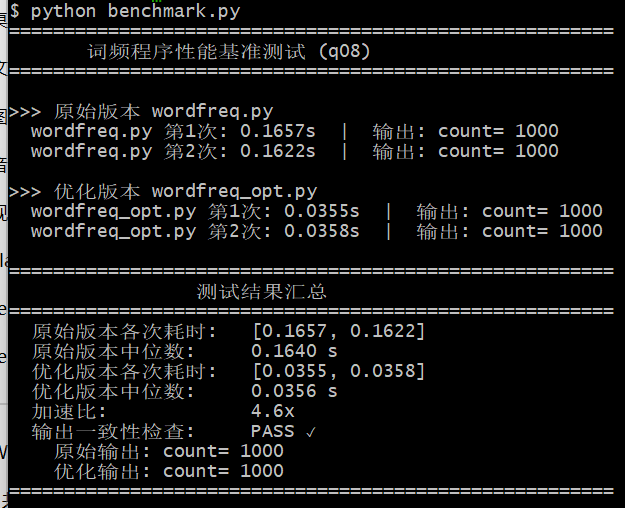
\includegraphics[width=0.9\textwidth]{实验四计算结果.png}
    \captionsetup{labelfont={color=themeBlue,bf}, textfont={color=darkText}}
    \caption{实验四:计算结果}
\end{figure}

% ==================== 课后思考题 ====================
\newpage
\section{课后思考题}

% ---------- 题 1 ----------
\subsection{思考题 1：特殊参数 \texttt{--} 与以短横线开头的文件名}
\textbf{题目}：理解命令 \texttt{cmd --flag -- --notaflag} 中 \texttt{--} 的作用。运行 \texttt{touch -- -myfile} 创建一个名为 \texttt{-myfile} 的文件，然后在不使用 \texttt{--} 的情况下尝试将其删除，观察现象并给出正确删除方法。

\textbf{解答}：
\texttt{--} 是一个特殊参数，用于告诉程序：\textbf{其后所有内容都不再作为选项（flag）解析}，一律视为位置参数（positional argument）。当文件名以 \texttt{-} 开头时（如 \texttt{-myfile}），\texttt{rm -myfile} 会被解析为 ``删除文件 \texttt{myfile} 并启用 \texttt{-f} 等选项''，从而报错 \texttt{invalid option}。解决方法有两种：使用 \texttt{rm -- -myfile}，或使用路径前缀 \texttt{rm ./-myfile} 使参数不以 \texttt{-} 开头。
\begin{lstlisting}
touch -- -myfile          # 创建文件
rm -myfile                # 错误示范（截图报错信息）
rm -- -myfile             # 正确删除
\end{lstlisting}
\begin{figure}[H]
    \centering
    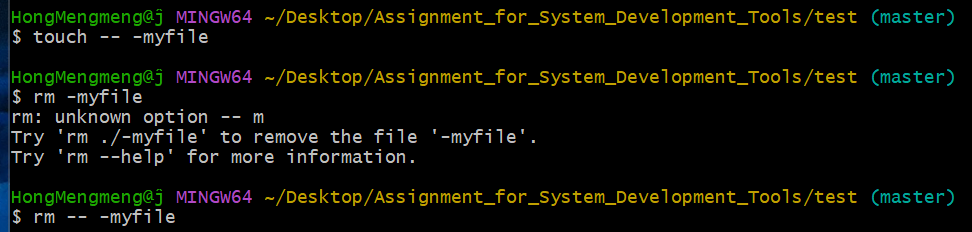
\includegraphics[width=0.9\textwidth]{思考题1.png}
    \captionsetup{labelfont={color=themeBlue,bf}, textfont={color=darkText}}
    \caption{思考题 1}
\end{figure}
% ---------- 题 2 ----------
\subsection{思考题 2：组合 \texttt{ls} 参数}
\textbf{题目}：阅读 \texttt{man ls}，写出一条 \texttt{ls} 命令，使其满足：(1) 包含所有文件（含隐藏文件）；(2) 文件大小以易读格式显示（如 454M）；(3) 按最近修改时间排序；(4) 输出带颜色。

\textbf{解答}：
通过查阅 \texttt{man ls} 可知各需求对应的选项为：
\begin{itemize}
  \item \texttt{-a}（\texttt{--all}）：列出所有文件，包括以 \texttt{.} 开头的隐藏文件；
  \item \texttt{-h}（\texttt{--human-readable}）：以 K、M、G 等单位显示文件大小（需配合 \texttt{-l} 才生效）；
  \item \texttt{-t}：按修改时间（mtime）排序，最近修改的排在最前；
  \item \texttt{-l}：长格式输出，显示权限、大小、时间等详细信息；
  \item \texttt{--color=auto}：为不同类型的文件着色（多数发行版的 \texttt{alias ls='ls --color=auto'} 已默认开启）。
\end{itemize}
\begin{lstlisting}
ls -ahtl --color=auto
\end{lstlisting}
\begin{figure}[H]
    \centering
    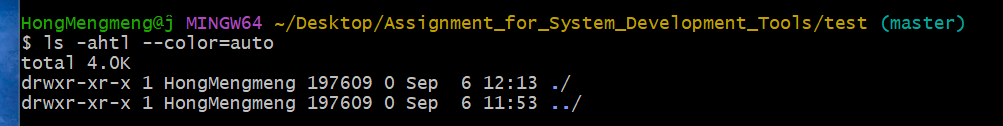
\includegraphics[width=0.9\textwidth]{思考题2.png}
    \captionsetup{labelfont={color=themeBlue,bf}, textfont={color=darkText}}
    \caption{思考题 2}
\end{figure}
% ---------- 题 3 ----------
\subsection{思考题 3：进程替换与 \texttt{printenv}、\texttt{export} 的区别}
\textbf{题目}：利用进程替换 \texttt{<(command)} 配合 \texttt{diff}，比较 \texttt{printenv} 与 \texttt{export} 的输出，并解释两者为什么不一样。

\textbf{解答}：
进程替换 \texttt{<(cmd)} 会把命令 \texttt{cmd} 的输出表现为一个文件描述符（实际是 \texttt{/dev/fd/63} 之类的临时文件），从而可以作为参数传给 \texttt{diff} 这类只接受文件的程序。执行 \texttt{diff <(printenv | sort) <(export | sort)} 后发现两者内容\textbf{本质相同但格式不同}：
\begin{itemize}
  \item \texttt{printenv} 输出的是当前进程的\textbf{环境变量}，格式为 \texttt{KEY=VALUE}；
  \item \texttt{export}（不带参数）输出的是当前 shell 中\textbf{被标记为导出的变量}，格式为 \texttt{declare -x KEY="VALUE"}，带有 \texttt{declare -x} 前缀和引号；
  \item 此外，\texttt{export -f} 导出的\textbf{shell 函数}也会出现在 \texttt{export} 的输出中（显示为 \texttt{declare -fx}），但函数并不属于环境变量，\texttt{printenv} 不会显示它们；
  \item 值中含有特殊字符时，\texttt{export} 会进行转义，而 \texttt{printenv} 原样输出。
\end{itemize}
因此差异主要来源于\textbf{输出格式}以及\textbf{导出函数}的存在，而非变量集合本身不同。
\begin{lstlisting}
diff <(printenv | sort) <(export | sort)
\end{lstlisting}
\begin{figure}[H]
    \centering
    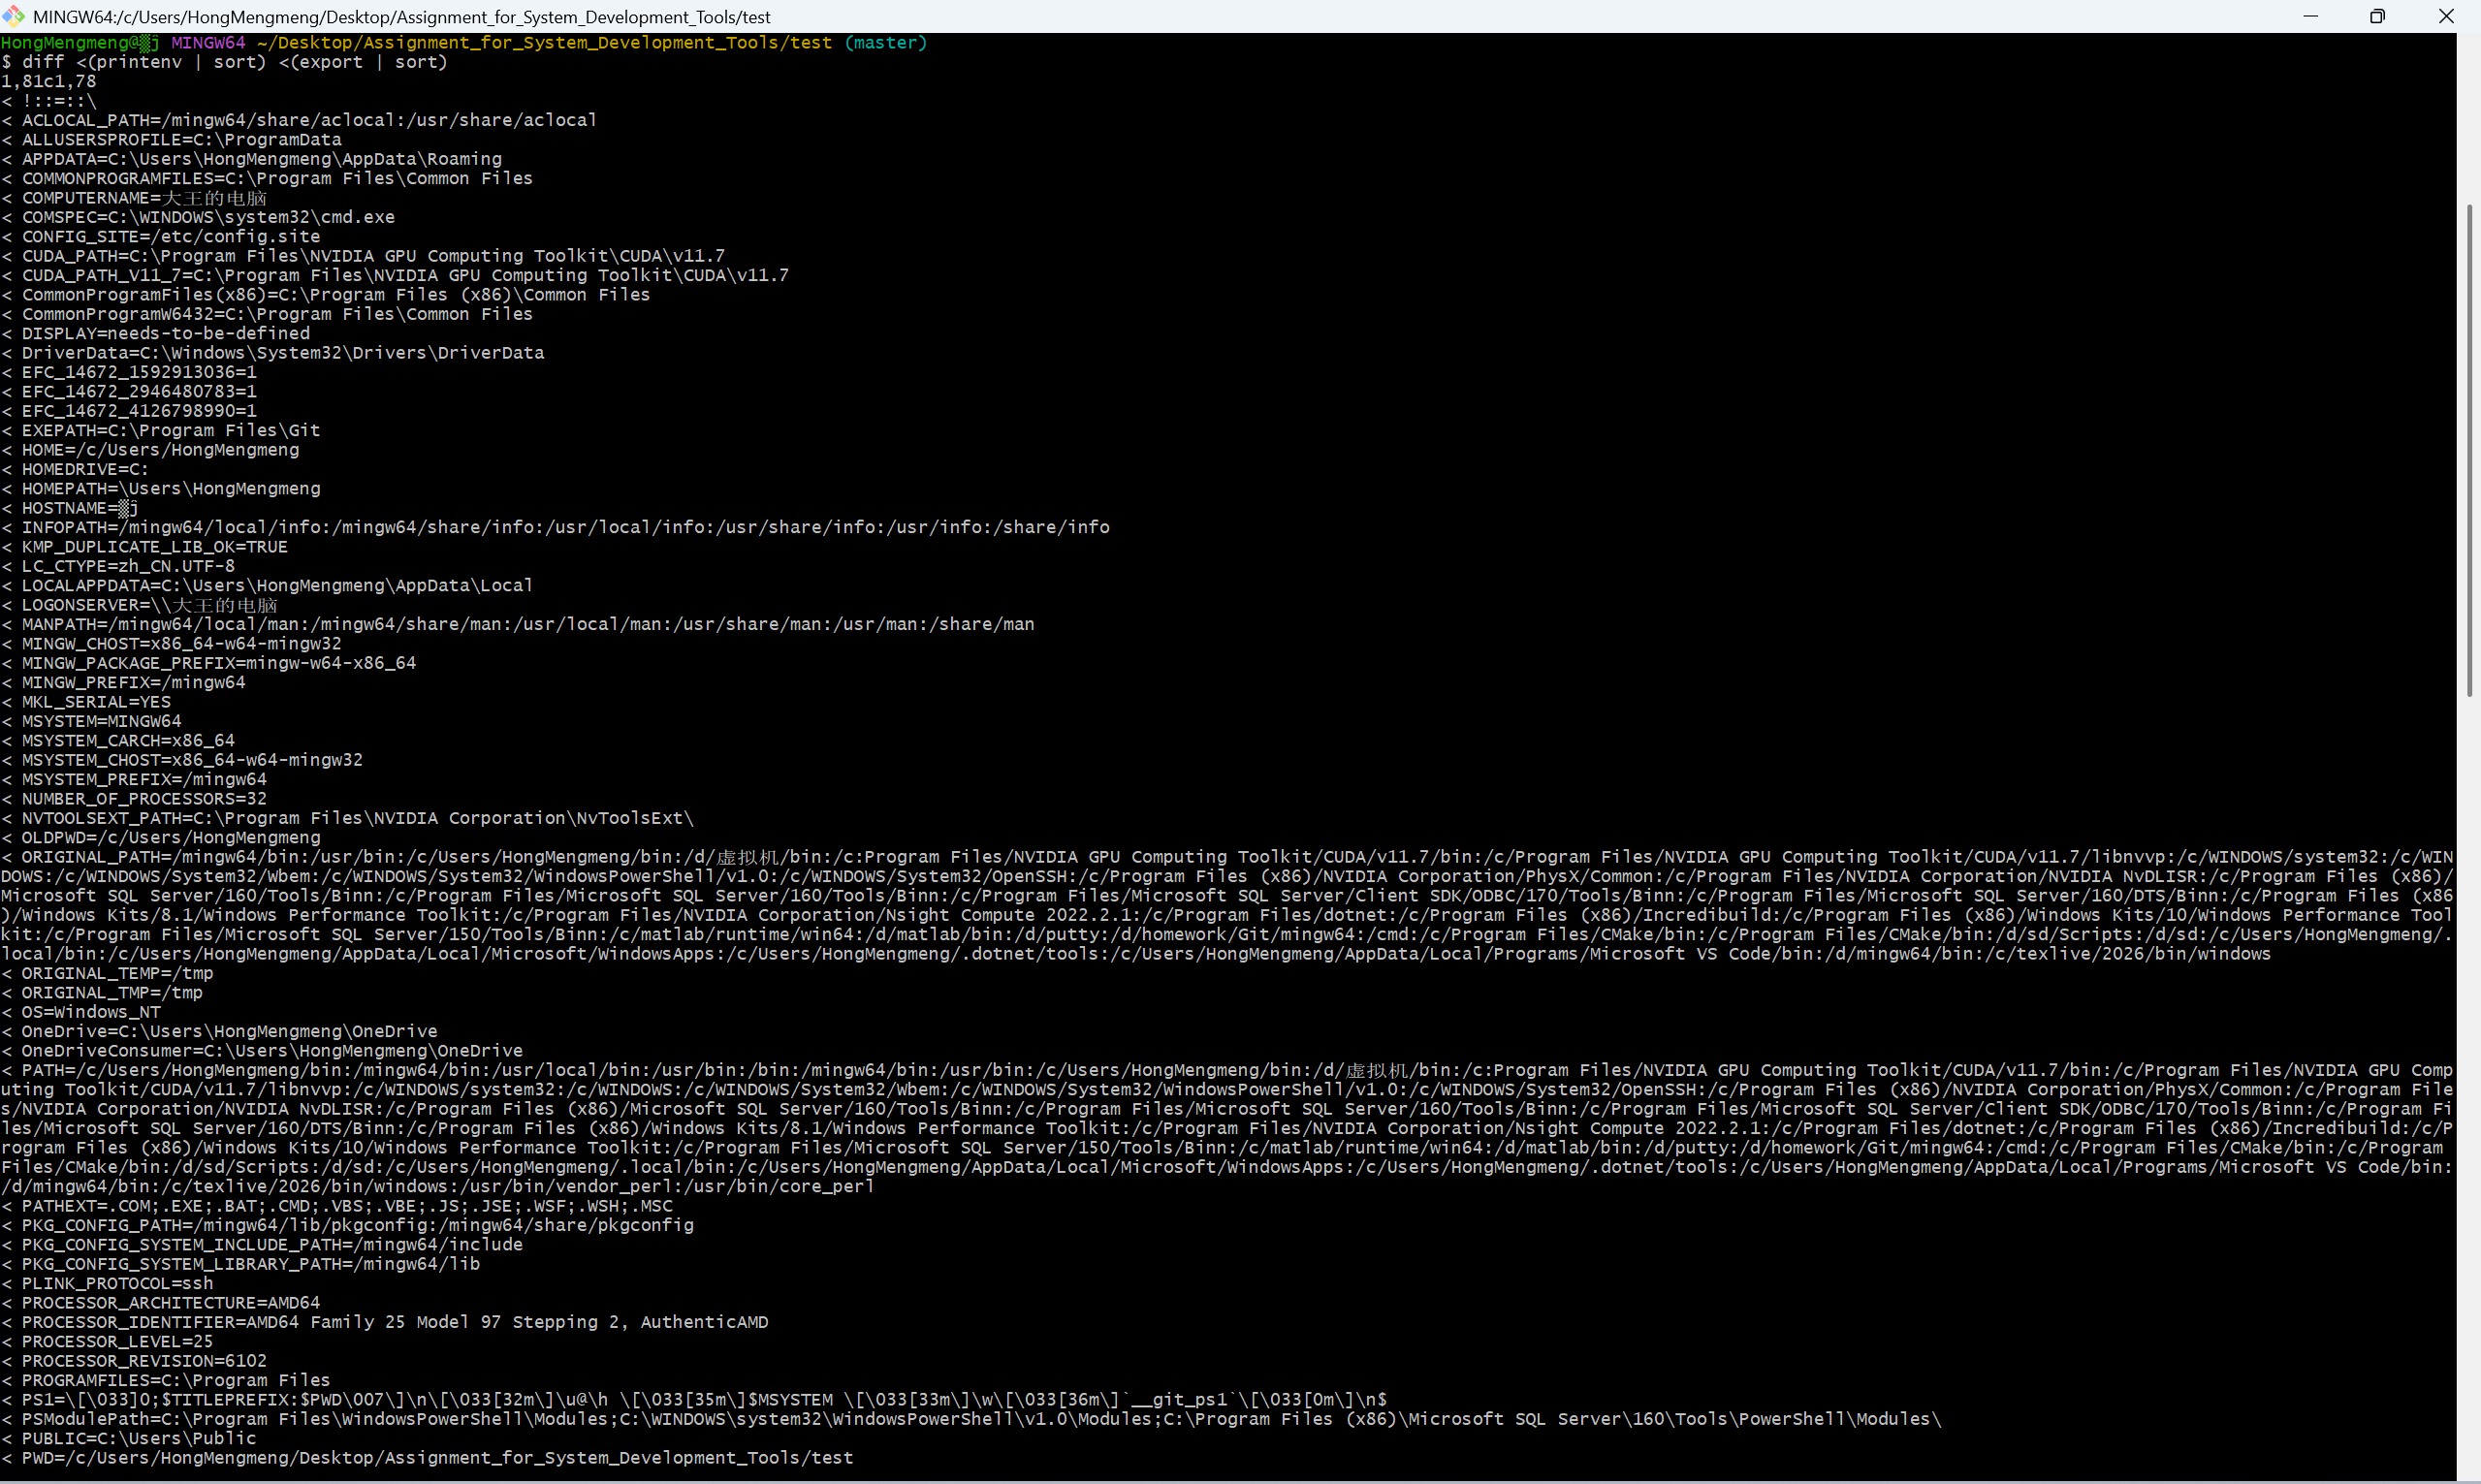
\includegraphics[width=0.9\textwidth]{思考题3.1.png}
    \captionsetup{labelfont={color=themeBlue,bf}, textfont={color=darkText}}
    \caption{思考题 3.1}
\end{figure}
\begin{figure}[H]
    \centering
    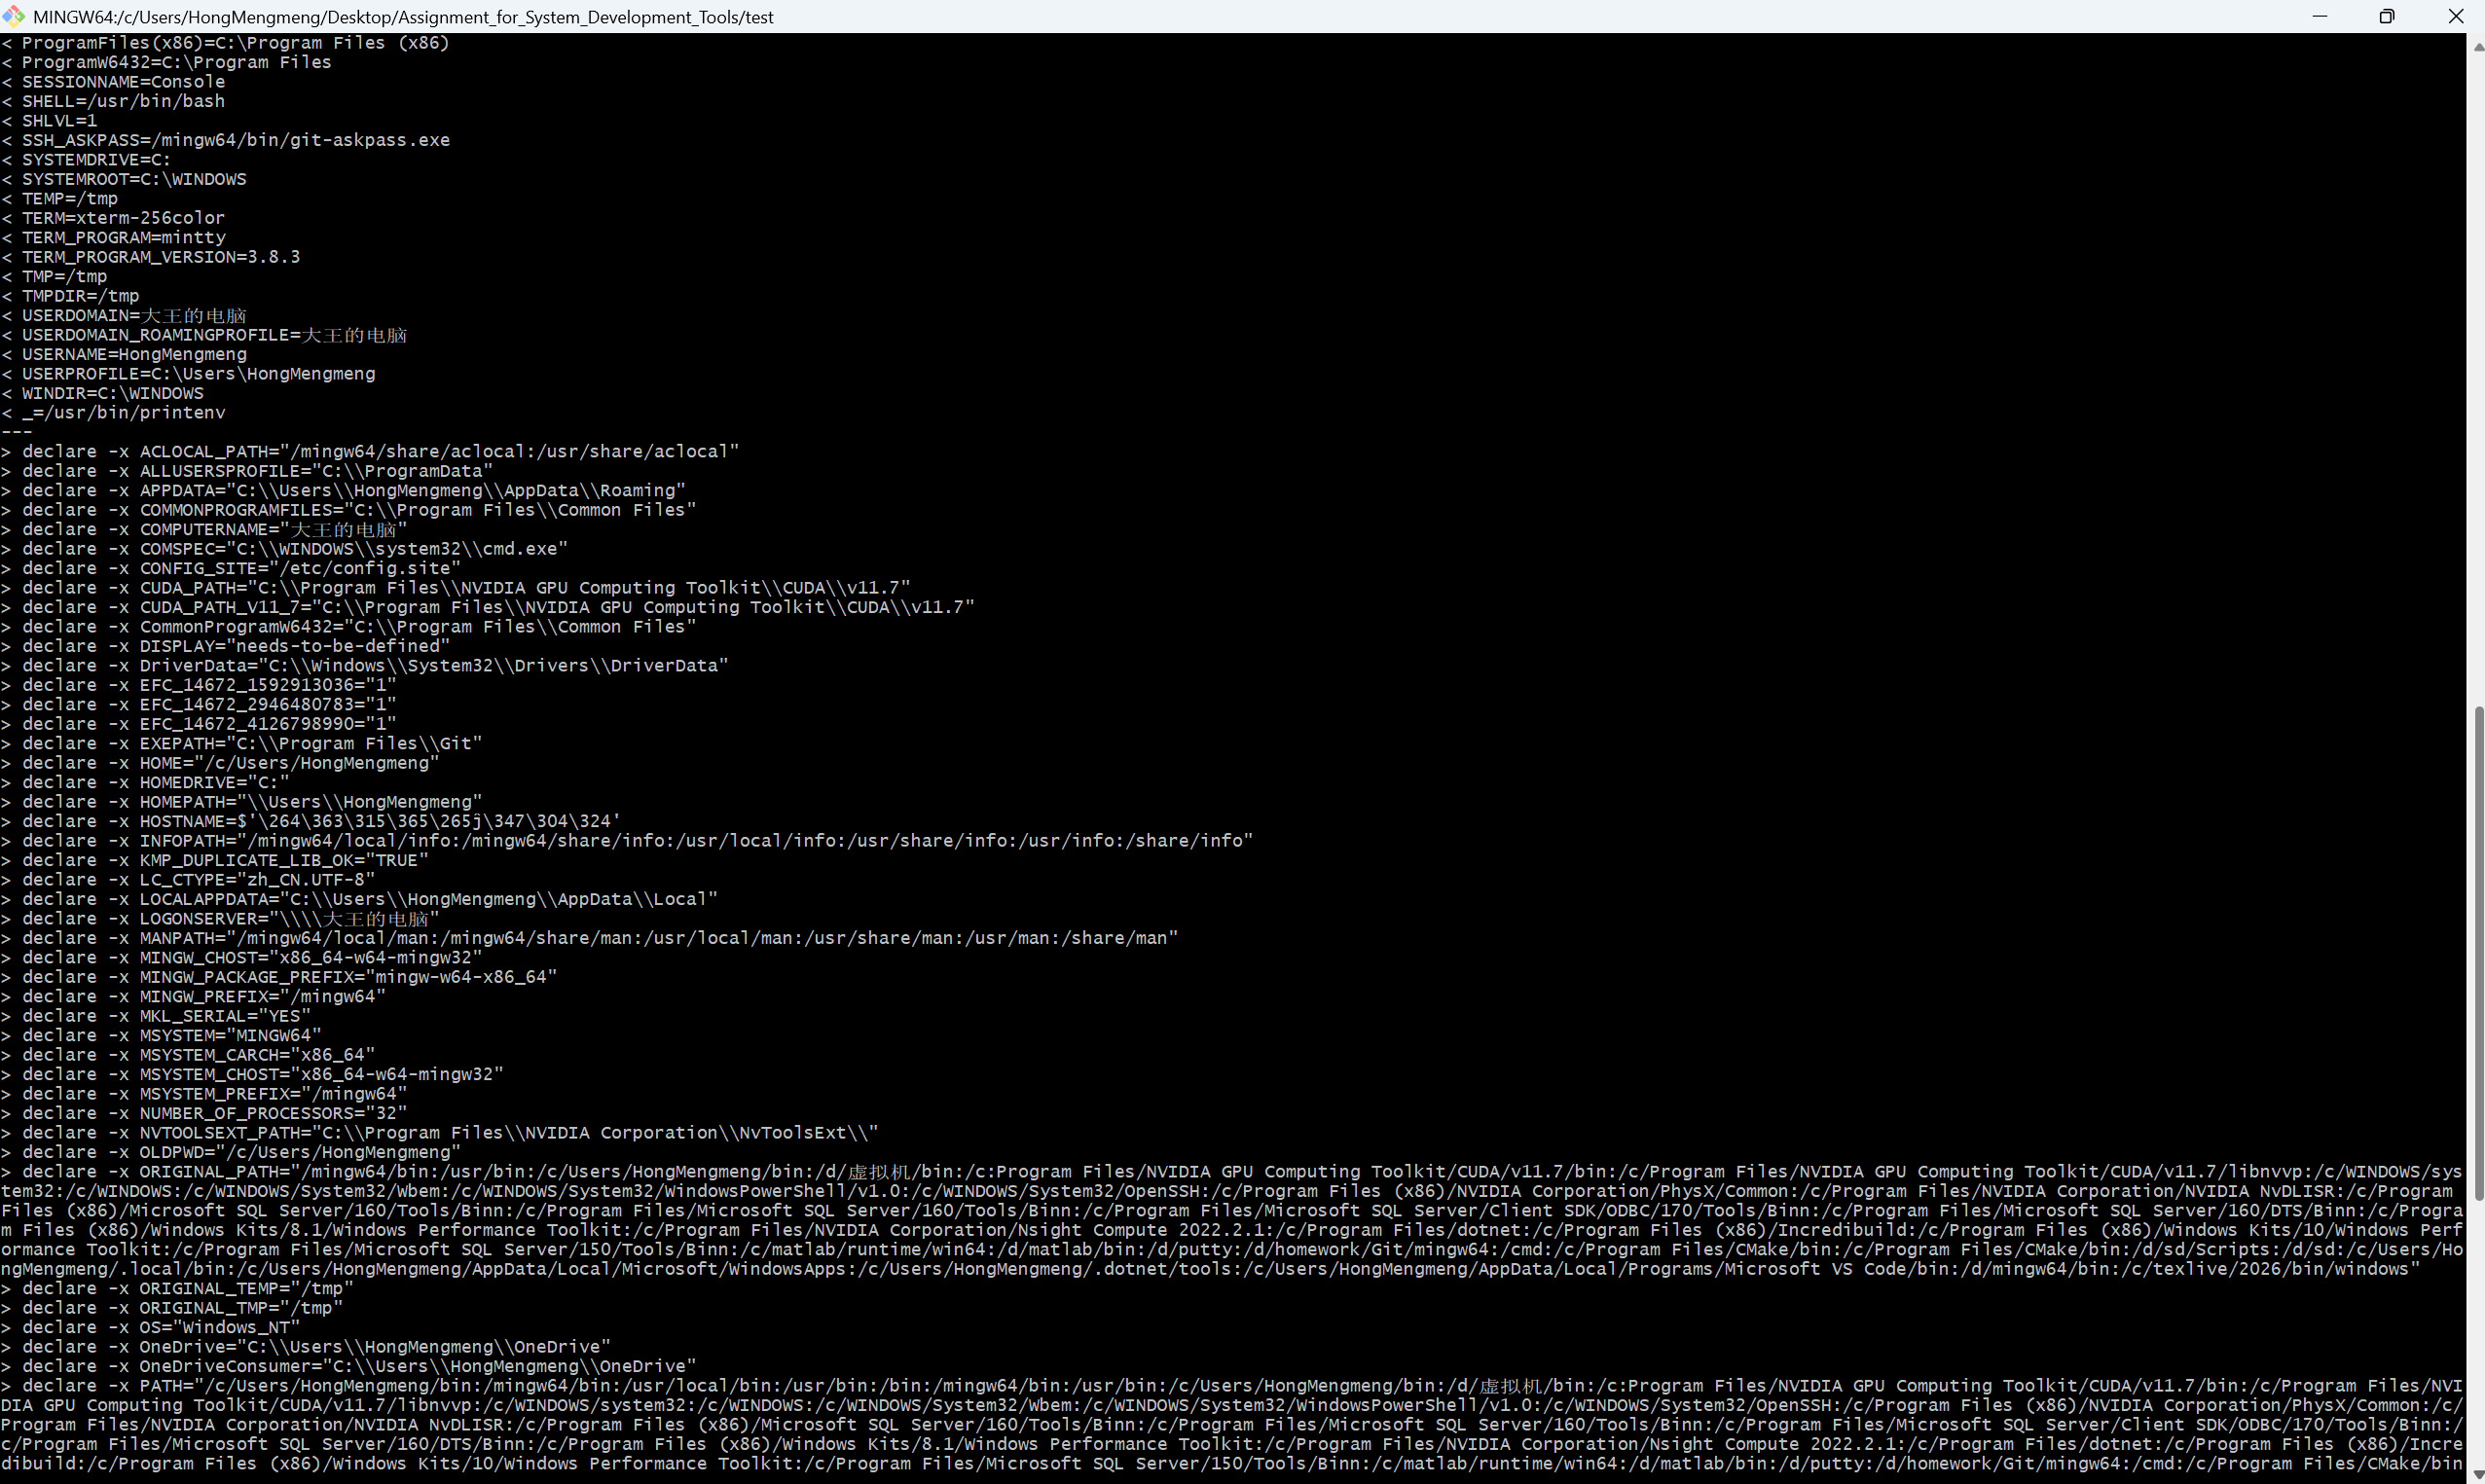
\includegraphics[width=0.9\textwidth]{思考题3.2.png}
    \captionsetup{labelfont={color=themeBlue,bf}, textfont={color=darkText}}
    \caption{思考题 3.2}
\end{figure}
\begin{figure}[H]
    \centering
    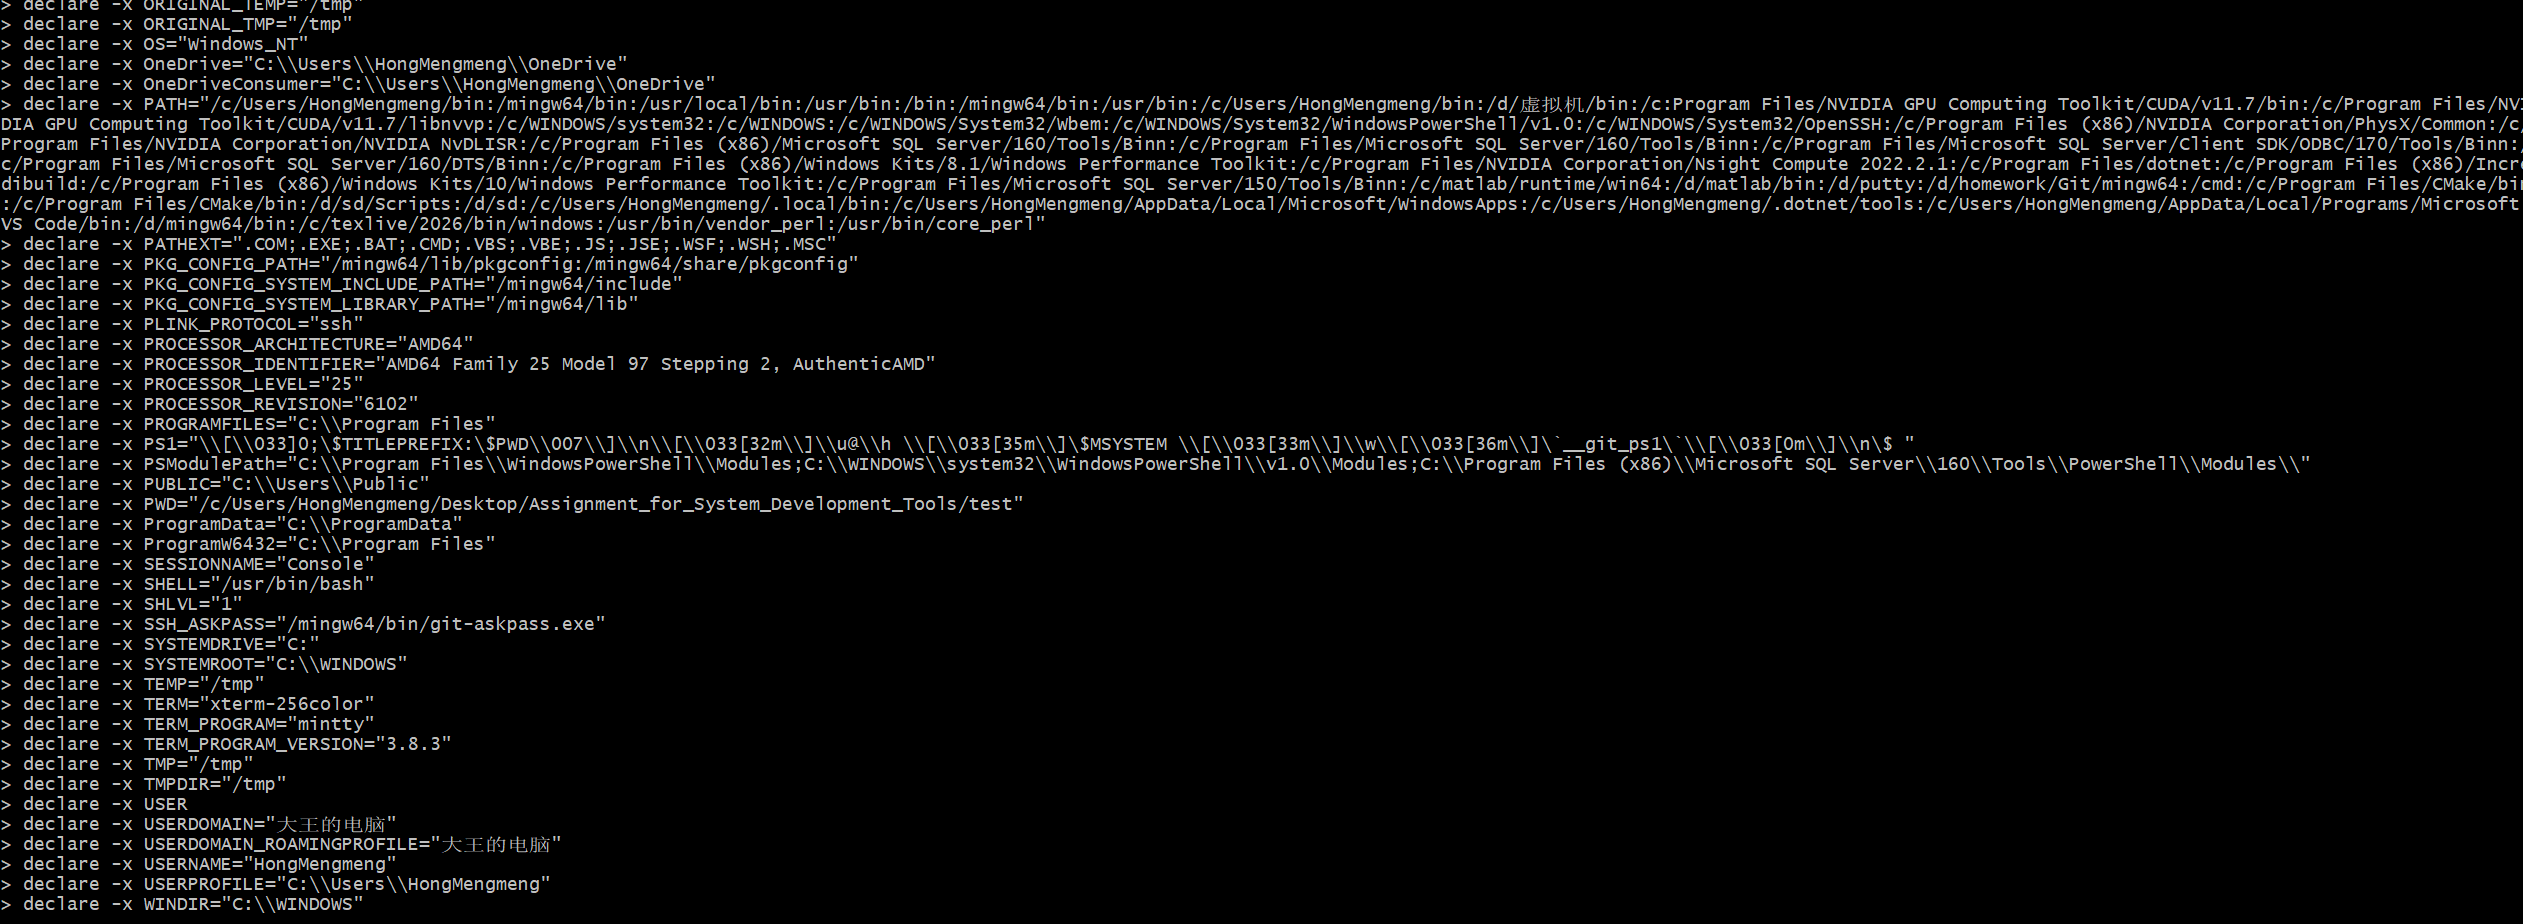
\includegraphics[width=0.9\textwidth]{思考题3.3.png}
    \captionsetup{labelfont={color=themeBlue,bf}, textfont={color=darkText}}
    \caption{思考题 3.3}
\end{figure}
% ---------- 题 4 ----------
\subsection{思考题 4：编写 \texttt{marco} 与 \texttt{polo} 函数}
\textbf{题目}：编写两个 bash 函数 \texttt{marco} 和 \texttt{polo}：执行 \texttt{marco} 时保存当前工作目录；此后无论切换到哪个目录，执行 \texttt{polo} 都能 \texttt{cd} 回执行 \texttt{marco} 时所在的目录。将代码写入 \texttt{marco.sh} 并通过 \texttt{source} 加载。

\textbf{解答}：
思路：用 \texttt{pwd} 获取当前目录并存入一个环境变量 \texttt{MARCO}，\texttt{polo} 再读取该变量执行 \texttt{cd}。关键点在于必须使用 \texttt{source marco.sh}（而非 \texttt{bash marco.sh}）来加载：因为 \texttt{source} 在\textbf{当前 shell} 中执行脚本，函数定义和变量修改才会保留；若用子进程运行脚本，退出后所有定义都会消失。另外，由于函数中用 \texttt{export} 导出了变量，即使进入子 shell 也能读取到保存的目录。

\texttt{marco.sh} 文件内容：
\begin{lstlisting}
#!/usr/bin/env bash
marco() {
  export MARCO="$(pwd)"     # 保存当前工作目录到环境变量
  echo "marco: saved $(pwd)"
}
polo() {
  cd "$MARCO" || echo "polo: MARCO not set, run marco first"
}
\end{lstlisting}

加载与测试：
\begin{lstlisting}
source marco.sh           # 加载函数
cd /tmp && marco          # 在 /tmp 打标记
cd / && polo && pwd       # 应输出 /tmp
\end{lstlisting}
\begin{figure}[H]
    \centering
    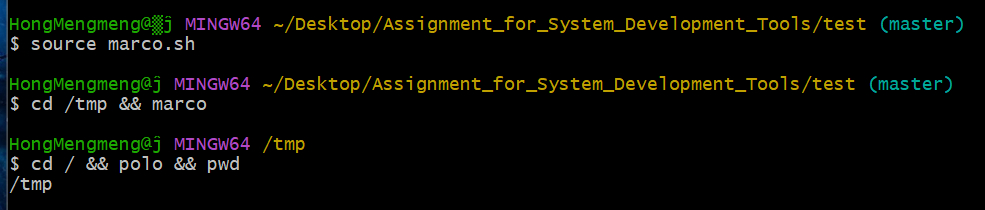
\includegraphics[width=0.9\textwidth]{思考题4.png}
    \captionsetup{labelfont={color=themeBlue,bf}, textfont={color=darkText}}
    \caption{思考题 4}
\end{figure}
% ---------- 题 5 ----------
\subsection{思考题 5：信号与任务控制（挂起、后台、\texttt{pgrep}、\texttt{pkill}）}
\textbf{题目}：在终端启动 \texttt{sleep 10000}，用 \texttt{Ctrl-Z} 挂起，再用 \texttt{bg} 使其在后台继续运行；然后使用 \texttt{pgrep} 找到其 pid，再用 \texttt{pkill} 将其杀掉，全程\textbf{不手动输入 pid}。

\textbf{解答}：
\texttt{Ctrl-Z} 向前台进程发送 \texttt{SIGTSTP} 信号将其挂起（状态变为 Stopped）；\texttt{bg} 使被挂起的任务在后台恢复运行（相当于发送 \texttt{SIGCONT}）。随后：
\begin{itemize}
  \item \texttt{pgrep -af sleep}：\texttt{-a} 显示完整命令行，\texttt{-f} 按整条命令行（而非仅进程名）匹配，便于确认找到的正是目标任务；
  \item \texttt{pkill -f "sleep 10000"}：按命令行模式匹配并默认发送 \texttt{SIGTERM} 将其终止，无需手动抄写 pid。使用带参数的模式 \texttt{"sleep 10000"} 而非单独的 \texttt{sleep}，可避免误杀系统中其他 \texttt{sleep} 进程。
\end{itemize}
\begin{lstlisting}
sleep 10000             
bg                     
ps aux | grep sleep
kill $(ps aux | grep "sleep 10000" | grep -v grep | awk '{print $2}')
\end{lstlisting}
\begin{figure}[H]
    \centering
    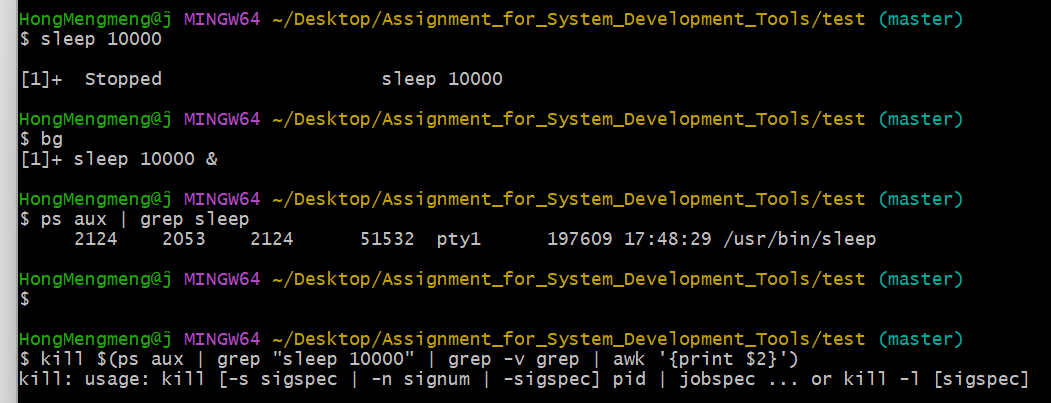
\includegraphics[width=0.9\textwidth]{思考题5.png}
    \captionsetup{labelfont={color=themeBlue,bf}, textfont={color=darkText}}
    \caption{思考题 5}
\end{figure}
% ---------- 题 6 ----------
\subsection{思考题 6：使用 \texttt{wait} 等待后台进程结束}
\textbf{题目}：在限制条件 \texttt{sleep 60 \&} 下，让一个 \texttt{ls} 等到该后台进程结束后再执行。

\textbf{解答}：
\texttt{wait} 命令会阻塞当前 shell，直到其\textbf{子进程}（后台任务）全部结束。因此只需在启动后台任务后执行 \texttt{wait}，再执行 \texttt{ls} 即可；也可以将三条命令用 \texttt{\&\&} 串联。注意 \texttt{wait} 只对\textbf{当前 shell 的子进程}有效：如果 \texttt{sleep} 是在另一个 bash 会话中启动的，本会话的 \texttt{wait} 无法等待它，这就引出了思考题 7 的 \texttt{pidwait}。
\begin{lstlisting}
sleep 60 &          # 后台启动
wait                # 阻塞直到后台任务结束（约 60 秒）
ls                  # sleep 结束后才执行
\end{lstlisting}
% ---------- 题 7 ----------
\subsection{思考题 7：编写 \texttt{pidwait} 函数等待任意 pid 结束}
\textbf{题目}：已知 \texttt{kill} 成功时退出状态为 0，失败时非 0；\texttt{kill -0} 不真正发送信号，仅检测进程是否存在。编写 bash 函数 \texttt{pidwait}，接收一个 pid，一直等待到该进程结束为止，并用 \texttt{sleep} 避免忙等浪费 CPU。

\textbf{解答}：
利用 \texttt{kill -0 pid} 的退出状态作为``进程是否存活''的判据：只要返回 0，说明进程仍存在，就 \texttt{sleep} 一小段时间后重试；一旦返回非 0（进程不存在或无权限），循环退出，函数返回。这种轮询方式对\textbf{非当前 shell 子进程}的 pid 同样有效，弥补了 \texttt{wait} 的局限。轮询间隔设为 1 秒，在响应速度与 CPU 开销之间取得平衡。

（\texttt{pidwait} 函数定义，可写入 \texttt{marco.sh} 一并 \texttt{source}）：

\begin{lstlisting}
pidwait() {
  while kill -0 "$1" 2>/dev/null; do
    sleep 1
  done
}
\end{lstlisting}

测试命令：
\begin{lstlisting}
source marco.sh
sleep 30 &                # 后台启动，记下 $! 的值
pidwait $!                # 等待该进程结束
echo "done"               # 约30秒后打印
\end{lstlisting}
\begin{figure}[H]
    \centering
    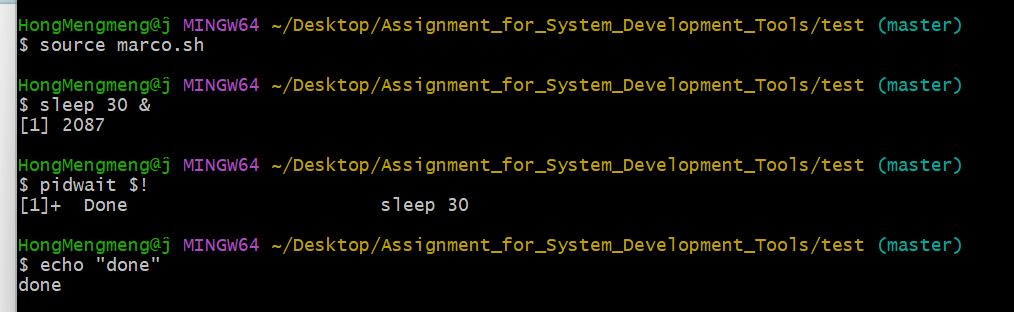
\includegraphics[width=0.9\textwidth]{思考题7.png}
    \captionsetup{labelfont={color=themeBlue,bf}, textfont={color=darkText}}
    \caption{思考题 7}
\end{figure}
% ---------- 题 8 ----------
\subsection{思考题 8：用 \texttt{pdb} 调试归并排序，定位 \texttt{merge} 中的取元素错误}
\textbf{题目}：按伪代码实现归并排序（实现中含有一个 bug），使用调试器逐步单步执行 \texttt{merge} 函数，找出错误元素被选中的位置并修复，使 \texttt{merge\_sort([3,1,4,1,5,9,2,6])} 返回 \texttt{[1,1,2,3,4,5,6,9]}。

\textbf{解答}：
用 Python 实现伪代码后直接运行，输出为乱序的 \texttt{[1, 5, 4, 3, 4, 6, 9]}，确认存在 bug。用 \texttt{pdb} 在 \texttt{merge} 函数上设断点并单步执行，观察 \texttt{i}、\texttt{j} 与 \texttt{result}：当 \texttt{left[i] > right[j]} 进入 \texttt{else} 分支时，代码写入的是 \texttt{right[i]} 而不是 \texttt{right[j]}。例如 \texttt{left=[1,3]}、\texttt{right=[1,4]} 时，\texttt{i=1, j=0}，本应取 \texttt{right[0]=1}，却取了 \texttt{right[1]=4}，导致顺序错乱。将 \texttt{right[i]} 改为 \texttt{right[j]} 后输出正确。

实现文件 \texttt{merge.py}（含 bug 的版本）：
\begin{lstlisting}
def merge(left, right):
    result = []
    i, j = 0, 0
    while i < len(left) and j < len(right):
        if left[i] <= right[j]:
            result.append(left[i]); i += 1
        else:
            result.append(right[i]); j += 1   # BUG: 应为 right[j]
    result.extend(left[i:])
    result.extend(right[j:])
    return result

def merge_sort(arr):
    if len(arr) <= 1:
        return arr
    mid = len(arr) // 2
    return merge(merge_sort(arr[:mid]), merge_sort(arr[mid:]))

print(merge_sort([3, 1, 4, 1, 5, 9, 2, 6]))
\end{lstlisting}

调试与修复命令：
\begin{lstlisting}
python merge.py                 # 输出 [1, 5, 4, 3, 4, 6, 9]，未排序，确认有 bug
python -m pdb merge.py          # 以 pdb 调试器启动
(pdb) break merge               # 在 merge 函数入口设断点
(pdb) continue                  # 每次进入 merge 都会停下
(pdb) print left, right         # 查看当前两半，重复 continue 直到 left=[1,3], right=[1,4]
(pdb) next                      # 单步执行，走进 else 分支
(pdb) print i, j, result        # j 仍指向未取的 1，result 中却被放入了 4
(pdb) print right[i], right[j]  # 对比：else 分支误取了 right[i]
(pdb) quit
# 将 merge.py 中 result.append(right[i]) 改为 result.append(right[j])
python merge.py                 # 输出 [1, 1, 2, 3, 4, 5, 6, 9]，修复成功
\end{lstlisting}
% ---------- 题 9 ----------
\subsection{思考题 9：用 gdb 定位 \texttt{uaf.c} 的释放后使用（UAF）}
\textbf{题目}：\texttt{uaf.c} 在 \texttt{free(greeting)} 之后仍对 \texttt{greeting} 进行写入与打印（释放后使用）。普通编译下程序"看似正常"，用 gdb 在 \texttt{free} 之后设断点并单步执行，定位非法访问行并修复。

\textbf{解答}：
普通编译运行输出两行问候，看似正常——这是因为释放后使用属于未定义行为，Windows 的堆管理器不一定立即回收或保护该内存页，所以不一定崩溃。用 gdb 在 \texttt{free} 调用之后设断点，单步执行到 \texttt{greeting[0]='J'} 时，可观察到对一个已释放地址进行写入；继续执行到第二条 \texttt{printf} 时读取的也是已释放内存。修复方法：删除 \texttt{free} 之后对 \texttt{greeting} 的所有访问（或将 \texttt{free} 移到所有使用之后）。

终端命令：
\begin{lstlisting}
gcc -g uaf.c -o uaf.exe
./uaf.exe                       # 输出两行，看似正常（UAF 未触发崩溃）
gdb ./uaf.exe
(gdb) break 10                  # 在第 10 行 free(greeting) 处设断点
(gdb) run                       # 运行到 free 停下
(gdb) print greeting            # 记录此时指针值，如 0x... 
(gdb) next                      # 执行 free，内存已释放
(gdb) next                      # 单步到 greeting[0]='J'，对已释放地址写入
(gdb) print greeting[0]         # 观察：写入发生在已 free 的内存上
(gdb) next                      # 单步到 printf，读取已释放内存
(gdb) quit
# 修复 uaf.c：删除 free 之后的 greeting[0]='J'; 与第二条 printf
gcc -g uaf.c -o uaf.exe && ./uaf.exe
                                # 修复后只输出 Hello, world!，无非法访问
\end{lstlisting}
\begin{figure}[H]
    \centering
    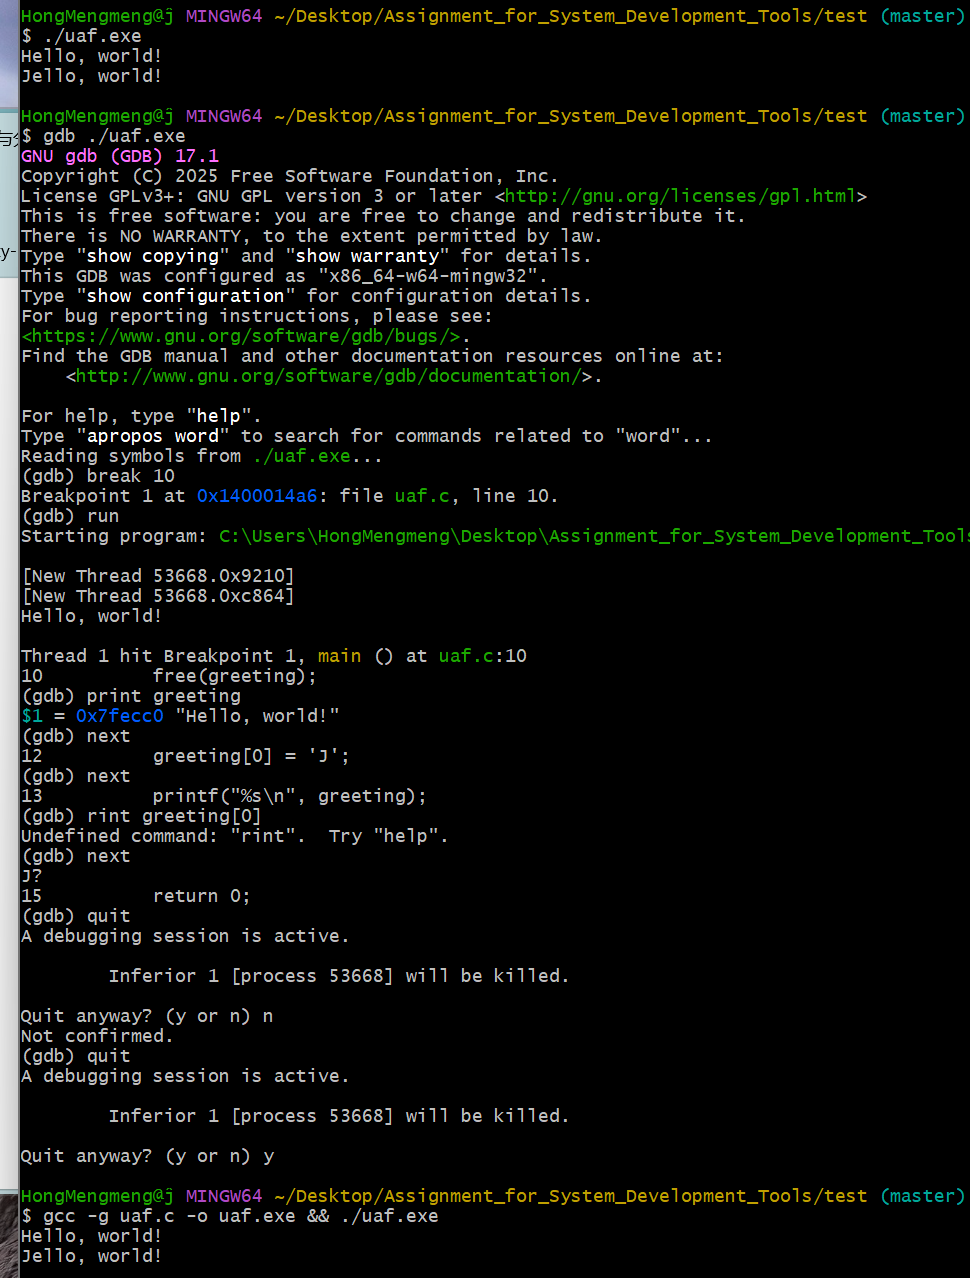
\includegraphics[width=0.9\textwidth]{思考题9.png}
    \captionsetup{labelfont={color=themeBlue,bf}, textfont={color=darkText}}
    \caption{思考题 9}
\end{figure}
% ---------- 题 10 ----------
\subsection{思考题 10：用 gdb 观察点定位 \texttt{corruption.c} 的越界写}
\textbf{题目}：编译运行 \texttt{corruption.c}，学生 1 的 ID 被损坏，但"肇事"函数 \texttt{curve\_scores} 表面上只修改学生 0。用 gdb 设置观察点找出究竟是哪一行覆盖了 \texttt{students[1].id}。

\textbf{解答}：
运行程序输出 \texttt{ERROR: Student 1's ID was corrupted! Expected 1002, got 1007}。原因是 \texttt{curve\_scores} 循环条件为 \texttt{i < 4}，而 \texttt{scores} 只有 3 个元素：当 \texttt{i=3} 时 \texttt{students[0].scores[3]} 越界写，由于结构体数组在内存中连续布局，该位置恰好是 \texttt{students[1].id}，被加 5 覆盖为 1007。对 \texttt{students[1].id} 设观察点后，程序自动停在越界写处，此时 \texttt{i==3}。修复：将循环条件改为 \texttt{i < 3}。

终端命令：
\begin{lstlisting}
gcc -g corruption.c -o corruption.exe
./corruption.exe                # 输出 ERROR，ID 变为 1007
gdb ./corruption.exe
(gdb) break main
(gdb) run
(gdb) next                      # 跨过 init()
(gdb) watch students[1].id      # 对学生 1 的 ID 设观察点
(gdb) continue                  # 自动停在越界写处：Old value=1002, New value=1007
(gdb) list                      # 显示停在 curve_scores 循环体内
(gdb) print i                   # i == 3，越界！
(gdb) quit
# 修复：将 curve_scores 中 i < 4 改为 i < 3
gcc -g corruption.c -o corruption.exe && ./corruption.exe
                                # 不再报 ERROR，输出正常
\end{lstlisting}
% ==================== 实验总结 ====================
\newpage
\section{实验总结与感悟}

\subsection{遇到的问题与解决方法}
\begin{enumerate}
    \item \textbf{Git Bash 缺少 \texttt{pgrep}/\texttt{pkill}}：思考题 5 中二者报 \texttt{command not found}（属 Linux 的 procps-ng 包）。改用 \texttt{kill \$(ps aux | grep "sleep 10000" | grep -v grep | awk '\{print \$2\}')} 动态取 PID 完成终止。
    \item \textbf{误以为 \texttt{wait} 让终端卡死}：思考题 6 中 \texttt{sleep 60 \&} 后接 \texttt{wait}，约一分钟无响应。另开终端用 \texttt{ps} 确认进程正常——\texttt{wait} 按设计阻塞至子进程退出，并非故障，改用 \texttt{sleep 5 \&} 快速验证后理解。
    \item \textbf{ASan/rr 不可用与 gdb 粘贴报错}：MinGW 不支持 \texttt{-fsanitize=address}，rr 仅支持 Linux，遂用 gdb 观察点 \texttt{watch students[1].id} 定位越界写、用断点单步定位 UAF；另发现从讲义复制命令进 gdb 会因不可见字符报 \texttt{Undefined command: ""}，改为手动键入即正常。
\end{enumerate}

\subsection{心得体会}
本次实验让我从"运行"进程进阶到"管理"进程：作业控制三件套与 \texttt{trap} 让我看清优雅退出与 \texttt{kill -9} 的本质差别，\texttt{wait} 与 \texttt{pidwait} 厘清了两种等待边界。调试上，\texttt{pdb} 单步让我亲眼看到 \texttt{right[i]} 与 \texttt{right[j]} 一字之差如何毁掉排序，gdb 观察点一句 \texttt{Old value=1002, New value=1007} 胜过反复加打印。实验四则教会我"先测量再优化"——用 \texttt{cProfile} 锁定热点，把 \texttt{list} 换 \texttt{set} 将 $O(n^2)$ 降为 $O(n)$。而 Git Bash 工具链的差异反而是一堂好课：工具因平台而异，但"观察—假设—验证"的方法处处通用。
\end{document}